
\documentclass[a4paper,14pt]{extarticle}

% Шрифты, кодировки, символьные таблицы, переносы
\usepackage{cmap}
\usepackage[T2A]{fontenc}
\usepackage[utf8x]{inputenc}
\usepackage[english, russian]{babel}

% Пакеты американского математического сообщества
\usepackage{amssymb,amsfonts,amsmath,amsthm}  
% Сокращения
\usepackage{cancel}

\theoremstyle{definition}
\newtheorem{definition}{Определение}

% Красная строка
\usepackage{indentfirst}

% Ссылки в pdf 
\usepackage[unicode, colorlinks, urlcolor=magenta, linkcolor=black]{hyperref}

% Таблицы
\usepackage{makecell,multirow} 

% Графика
\usepackage{graphicx}
\usepackage[usenames,dvipsnames]{color} 
\usepackage{float}
 \usepackage{xcolor}

% Геометрия страницы
\usepackage{geometry}
\geometry{left=2cm,right=2cm,top=2.5cm,bottom=2.5cm,bindingoffset=0cm,headheight=18pt}

% Колонтитулы
\usepackage{fancyhdr} 
% применим колонтитул к стилю страницы
\pagestyle{fancy} 
%очистим "шапку" страницы
\fancyhead{} 
%слева сверху на чётных и справа на нечётных
\fancyhead[R]{Лекции В.И. Некоркина 2018-2019} 
% \fancyhead[R]{Сарафанов Ф.Г., Понур К.А. и др.} 
%справа сверху на четных и слева на нечетных
\fancyhead[L]{Теория колебаний} 
%очистим "подвал" страницы
\fancyfoot{} 
% номер страницы в нижнем колонтитуле в центре
\fancyfoot[C]{\thepage} 

% Междустрочный отступ
\usepackage{setspace}
\linespread{1.15} % капельку увеличенный
\frenchspacing % <<французские>> пробелы

% Нумерация
\renewcommand{\labelenumii}{\theenumii)}
% В заголовках появляется точка, но при ссылке на них ее нет
\usepackage{misccorr}

% Содержание
\usepackage{tocloft}
\usepackage{secdot}
\sectiondot{subsection}

% Физика
\usepackage{physics}

% Новые команды
\newcommand{\Mean}[1]{\langle#1\rangle}
\newcommand{\Defi}{\underset{def}{=}}
\newcommand{\Inte}{\int\limits_{-\infty}^{\infty}} 
\newcommand{\const}{\textrm{const}}

\renewcommand{\div}{\textrm{div}}
\renewcommand{\grad}{\textrm{grad}}
\newcommand{\rot}{\textrm{rot}}

\addto\captionsrussian{%
	\renewcommand{\contentsname}{Оглавление}
	\renewcommand{\partname}{Раздел}%
}
\def\thepart{\arabic{part}}
\usepackage{tocloft}
\renewcommand{\cftpartleader}{\cftdotfill{\cftdotsep}} % for parts
\renewcommand{\cftsecleader}{\cftdotfill{\cftdotsep}} % for chapters
\renewcommand\thepart{\arabic{part}.}

\renewcommand{\cftsecaftersnum}{.}

\renewcommand{\cftsecdotsep}{\cftdotsep}
\renewcommand{\kappa}{\varkappa}
\renewcommand{\phi}{\varphi}
\renewcommand{\epsilon}{\varepsilon}
\renewcommand{\vec}{\mathbf}
% #1: math symbol
% #2: legend
\def\alegend#1#2{\overset{\underset{\scriptstyle\downarrow}{\scriptstyle\text{#2}}}{#1}}
\def\blegend#1#2{\underset{\underset{\scriptstyle\text{#2}}{\scriptstyle\uparrow}}{#1}}
\def\hp{\hat{p}}
\def\hx{\hat{x}}
\def\hH{\hat{H}}

\usepackage[explicit]{titlesec}
\usepackage{epigraph}


% \newcommand\praktika[1]{
% \stepcounter{section}
% \vspace{1.5em}
% \noindent\textbf{\Large{Занятие \arabic{section}.\hspace{.2em} #1}}
% % \newline 
% \vspace{-0.5em}
% \addcontentsline{toc}{section}{Занятие \arabic{section}.\hspace{.5em} #1}
% }

\usepackage{mathtools}
\mathtoolsset{showonlyrefs=true}


% https://tex.stackexchange.com/questions/8720/overbrace-underbrace-but-with-an-arrow-instead

\usepackage{xparse}% http://ctan.org/pkg/xparse

\NewDocumentCommand{\overarrow}{O{=} O{\uparrow} m}{%
  \overset{\makebox[0pt]{\begin{tabular}{@{}c@{}}$#3$\\[0pt]\ensuremath{#2}\end{tabular}}}{#1}
}
\NewDocumentCommand{\underarrow}{O{=} O{\downarrow} m}{%
  \underset{\makebox[0pt]{\begin{tabular}{@{}c@{}}\ensuremath{#2}\\[0pt]$#3$\end{tabular}}}{#1}
}

\newcommand\undernoteqty[2]{
	%
	\underarrow[
		\qty(\underbrace{#1})
	][\uparrow]{\substack{#2}}
	%
}

\newcommand{\pvec}[1]{\vec{#1}\mkern2mu\vphantom{#1}}
% Нормальный вектор для штрихов
\newcommand{\phat}[1]{\hat{#1}\mkern2mu\vphantom{#1}}

\newcommand\undernote[2]{
	%
	\underarrow[
		#1
	][\uparrow]{\substack{#2}}
	%
}


% Настройки для inkscape
\graphicspath{{fig/}} % путь, где искать картинки
% следующий код взят из 
% http://mirrors.ctan.org/info/svg-inkscape/InkscapePDFLaTeX.pdf
% \newcommand{\executeiffilenewer}[3]{%
    % \ifnum\pdfstrcmp{\pdffilemoddate{#1}}%
    % {\pdffilemoddate{#2}} > 0 %
    % {\immediate\write18{#3}}\fi}
\newcommand{\includesvg}[1]{%
    % \executeiffilenewer{#1.svg}{#1.pdf}
    % \immediate\write18{D:/Inkscape/inkscape --file=fig/fig1_2.svg --export-pdf=fig/fig1_2.pdf --export-latex > output}%
    % \input{#1.pdf_tex}%
  }
%-----------------------------------
% ##############################################################################
\newcommand*\dotvec[1][1,1]{\crossproducttemp#1\relax}
\def\crossproducttemp#1,#2\relax{{\qty[\vec{#1}\times\vec{#2}\,]}}

\newcommand*\prodvec[1][1,1]{\crossproducttempa#1\relax}
\def\crossproducttempa#1,#2\relax{{\qty[{#1}\times{#2}\,]}}
% ##############################################################################
% \usepackage{kbordermatrix}%
% \renewcommand{\kbldelim}{(} % change default array delimiters to parentheses
% \renewcommand{\kbrdelim}{)}
\newcommand{\markerr}{\textcolor{red}{\textbf{??}}} 
\usepackage{wrapfig,dsfont}
\usepackage{chngcntr}

\counterwithin*{equation}{section}
\begin{document}
%!TEX root = lections.tex
\begin{titlepage}
\thispagestyle{empty}

\begin{center}
	{\small\textsc{Нижегородский государственный университет имени Н.\,И. Лобачевского}}
	\vskip 3pt \hrule \vskip 5pt
	{\small\textsc{Радиофизический факультет}}

	\vfill

	\begin{spacing}{2}
	% {\huge \bf  Курин\, В.В.}\\[1.5em]
	{\Huge \bf  Лекции по теории колебаний}\\%\vspace{1em}
	\end{spacing}
	\vspace{1em}
	{ Набор и вёрстка:}\\[.5em]
	{ 
		\href{https://github.com/AnnaKarusevich}{\color{black}{Карусевич А.А.}},
		\href{https://github.com/fedorsarafanov}{\color{black}{Сарафанов Ф.Г.}}}\\[2em]
	% {\large }\\
	\vspace{1em}
\end{center}

\textbf{Disclaimer.} В данном документе нами набраны лекции по теории колебаний (нелинейной динамике), прочитанные на 3 курсе радиофизического факультета ННГУ \textbf{Владимиром Исааковичем Некоркиным}, но не вошедшие в сущестующие методические пособия. Документ призван облегчить подготовку к зачётам и экзаменам и восполнить пробелы в знаниях читателя по теории колебаний. Разрешено копирование и распространение данного документа с обязательным указанием первоисточника. 

При обнаружении ошибок, опечаток и прочих вещей, требующих исправления, можно либо создать issues в \href{https://github.com/FedorSarafanov/NonlinearDynamics}{репозитории на github.com}, либо написать на электронную почту  \href{mailto:sfg180@yandex.ru}{\color{black}{sfg180@yandex.ru}}.

\begin{center}
	\vfill
	4 апреля -- \today\\Нижний Новгород
\end{center}

\end{titlepage}


\newpage
\tableofcontents 
\newpage
\section{Введение в теорию колебаний}
\label{sec:lect1}
	%!TEX root = ../lections.tex
\newcommand{\R}{\mathbb{R}}
\newcommand{\Z}{\mathbb{Z}}
\section{Общие закономерности теории колебаний} % (fold)

Колебательные процессы и системы настолько широко распространены в
природе, технике и обществе, что любой из нас с ними неоднократно
сталкивается в повседневной жизни и, по-видимому, без труда сформулирует
основные их свойства. Действительно, когда мы слышим о колебаниях
температуры, курса валют, электрического напряжения, маятника, уровня воды
и так далее, нам понятно, что речь идет о процессах во времени или в
пространстве, обладающих той или иной степенью повторяемости и
возвращаемости к начальному или близкому состояниям. Причем, эти базовые
свойства процессов не зависят от природы систем и поэтому могут быть
описаны и изучены с единой точки зрения в рамках общего
междисциплинарного подхода. Именно такой подход и развивает теория
колебаний, предметом которой являются колебательные явления и процессы в
системах различной природы. Колебательные свойства реальных систем теория
колебаний получает из анализа соответствующих моделей. В результате такого
анализа устанавливается связь между параметрами модели и её
колебательными свойствами.

Теория колебаний является как прикладной, так и фундаментальной
наукой. Прикладной характер теории колебаний определяется её
многочисленными приложениями в физике, механике, автоматическом
управлении, радиотехнике и электронике, приборостроении и т.д. В этих
областях науки методами теории колебаний проведено исследование большого
числа различных систем и явлений. Более того, на базе теории колебаний
возникли новые технические направления – вибротехника, вибродиагностика,
биомеханика и др. Фундаментальный характер теории колебаний заключен в
самих моделях, которые она изучает. Это так называемые динамические
системы, с помощью которых можно описать любую детерминированную`'
эволюцию во времени или во времени и пространстве. Именно изучение
динамических систем позволило теории колебаний ввести понятия и
положения, развить методы и получить результаты, оказывающие большое
влияние на другие естественные науки. Здесь достаточно отметить
линеаризованную теорию устойчивости, понятия автоколебаний и резонанса,
теорию бифуркаций, хаотические колебания и др.
% subsection общие_закономертности_теории_колебаний (end)

\section{Динамические системы} % (fold)
Рассмотрим систему, состояние которой определяется вектором $\vec x (t) 
\in \R^n$. Предположим, что эволюция системы определяется одно-параметрическим семейством операторов $G^t$, $t\in\R$ (или $t\in\R^+$) или $t\in \Z$ (или $t\in\Z^+$), таких, что состояние системы в момент $t$
\begin{equation}
	\label{eq:1.1}
	\vec x(t,\vec x_0) = G^t \vec x_0,
\end{equation}
где $\vec x_0$ -- начальное состояние (начальная точка). Предположим также, что эволюционные операторы удовлетворяют двум следующим свойствам, отражающим детерминистический характер описываемых процессов.
\begin{enumerate}
	\item $G^0$ -- тождественный оператор, т.е.
	\begin{equation}
	\label{eq:1.2}
		\vec x(0, \vec x_0), \text{ для любых } \vec x_0.
	\end{equation}

Это свойство означает, что состояние системы не может изменяться самопроизвольно.

	\item  Второе свойство эволюционных операторов имеет вид:
	\begin{equation}
		\label{eq:1.3}
		G^{t_1+t_2}= G^{t_1} \circ G^{t_2}= G^{t_2} \circ G^{t_1},
	\end{equation}
	т.е.
	\begin{equation}
		\label{eq:1.4}
		\vec x (t_1+t_2, \vec x_0) = \vec x (t_1, \vec x(t_2, \vec x_0)) = \vec x (t_2, \vec x (t_1,x_0))
	\end{equation}
\end{enumerate}
 
 Согласно \eqref{eq:1.3} система приходит в одно и то же финальное состояние независимо от того, достигается ли оно за один временной интервал $t_1+t_2$, или за несколько последовательных интервалов $t_1$ и $t_2$, суммарной равных $t_1+t_2$.

 Совокупность всех начальный точек $X$ или всех возможных состояний системы (в рассматриваемом случае $X= \R^n$) называется фазовым пространством, а пара $\qty(X,\{G^t\})$, где семейство эволюционных операторов удовлетворяют условиям \eqref{eq:1.3} - \eqref{eq:1.2}, -- динамической системой (ДС).

 ДС делятся на два важных класса -- с непрерывным временем, если $t\in \R$ или $\R_+$,  и с дискретным временем, если $t\in \Z$ или $\Z_+$.

 Эволюция системы соответствует движению изображающей точки в фазовом пространстве вдоль траектории $\Gamma = \bigcup\limits_t G^t \vec x_0$. Семейство $ \Gamma^+ = \bigcup\limits_{t\geq 0} G^t \vec x_0 $\quad  $ \qty(\Gamma^- = \bigcup\limits_{t< 0} G^t \vec x_0)$ называется положительной (отрицательной) полутраекторией, проходящей через начальную точку $\vec x_0$. Если семейство $\{G^t\}$ является непрерывным по $t$ (для ДС с непрерывным временем ), то траектории (полутраектории) представляют собой непрерывные кривые в $X$. Для ДС с дискретным временем траектории являются дискретными подмножествами в фазовом пространстве.

 Введем необходимое в дальнейшем понятие инвариантности множества.
 Множество $A \subset X$ называется положительно (отрицательно) инвариантным , если оно состоит из положительных полутраекторий, т.е. $A$ - положительно (отрицательно) инвариантно, если $G^t A \subset A, t>0 ~ (t<0)$. Множество $A$ называется инвариантным, если оно одновременно инвариантно как положительно, так и отрицательно.	


\subsection{Типы траекторий} % (fold)
\label{subsubsec:1.2.1}
Дадим определение основных типов траекторий ДС.
\begin{itemize}
	\item Точка $\vec x_0$ называется неподвижной точкой ДС, если $G^t \vec x_0 = \vec x_0$ для всех $t$ (для систем с непрерывным временем такие точки чаще называют состояниями или положениями равновесия).
	\item Точка $\vec x_0$ называется периодической, если существует такое $T>0$ , что $G^t \vec x_0 = \vec x_0$ и $G^t \vec x_0 \neq \vec x_0$ для $0<t<T$, а соответствующая траектория $\bigcup\limits_{0\leq t \leq T} G^t \vec x_0$ динамической системы, проходящая через эту точку -- периодической. Периодическая траектория является замкнутой кривой в фазовом пространстве ДС с непрерывным временем и совокупностью $T$-периодических точек для ДС с дискретным временем.
	\item Точка $\vec x_0$ называется неблуждающей, если для любой окрестности открытого множества $U \ni \vec x_0$ этой точки и любого $t_0>0$ найдется сколь угодно большое $t>t_0$, такое что $G^t U \cap U \neq \varnothing $. Траектория, проходящая через такую точку, называется неблуждающей. 
\end{itemize}

Между траекториями ДС и движениями реальных систем существует соответствие. Неподвижным точкам ДС отвечают стационарные состояния реальных систем, периодическим траекториям -- периодические движения, а неблуждающим траекториям -- движения с некоторым повторением их состояний во времени.

Заметис, что вышеприведенные траектории могут существовать и в ДС, у которых фазовое пространство не обязательно $\R^n$. Например, фазовым пространством динамической системы, описывающей колебания математического маятника является цилиндр $X= S^1 \times \R $, поскольку состояние маятника в любой момент времени однозначно описывается значением угловой переменной $\phi(t)$, определенной с точностью до $2\pi ~ (\phi \in S^1)$  значением её скорости $\dot \phi \in \R$.
% subsubsection типы_траекторий (end)

\subsection{Динамические системы с непрерывным временем} % (fold)
Для многих ДС с непрерывным временем правило, которое позволяет найти состояние в любой момент времени по начальному состоянию, задается системой обыкновенных дифференциальных уравнений
\begin{equation}
	\dot x_i = f_i (x_1,x_2,\dots, x_N), ~ i = 1,2, \dots, N
\end{equation}
или в векторной форме
\begin{equation}
	\label{eq:1.5}
	\vec {\dot x_i} = \vec F (\vec x), ~ \vec x \in \R^n, ~ \vec F: \R^n \rightarrow \R^n,
\end{equation}
для которой условия существования и единственности решений выполнены (здесь и далее мы будем обозначать точкой дифференцирование по времени). В этом случае семейство $G^t \vec x_0$ задается просто решением системы \eqref{eq:1.5} с начальным условием $\vec x(0, \vec x_0)= \vec x_0$. Например, для линейной системы
\begin{equation}
	\dot {\vec x} = A \vec x,
\end{equation} 
где $A$ -- матрица размерности $n \times n $ с постоянными коэффициентами, решение имеет вид $\vec x(t, \vec x_0)= e^{At} \vec x_0$, в котором $e^{At}$ -- матрица $n \times n$. Поскольку матрицы $e^{A_1t}$ и $e^{A_2t}$ коммутируют для любой пары $t_1, t_2$, то свойство \eqref{eq:1.3}:
\begin{equation}
	e^{A(t_1+t_2)}= e^{At_1}\circ e^{At_2} = e^{At_2}\circ e^{At_1} 
\end{equation}
выполняется. Свойство \eqref{eq:1.2} также, очевидно, выполнено.

В качестве другого примера рассмотрим систему, заданную в полярных координатах
\begin{equation}
	\dot \rho = \lambda \rho, \quad \dot \phi = \omega
\end{equation}
Следовательно, эволюционные операторы задаются следующим образом
\begin{equation}
	G^t:\quad (\rho_0,\phi_0) \rightarrow (\rho_0 e^{\lambda t}, \omega t + \phi).
\end{equation}
Очевидно, что свойства \eqref{eq:1.2}-\eqref{eq:1.3} выполняются.

Обратим внимание н ато, что правая часть системы \eqref{eq:1.5} явно от времени не зависит. Такие системы называются \textbf{автономными}. Существует также большое число задач (например, системы, подверженные внешнему переменному силовому воздействие), описываемых динамическими системами, правые части которых явно зависят от времени. Они называются \textbf{неавтономными}.

% subsubsection динамические_системы_с_непреры (end)

\subsection{Динамические системы с дискретным временем} % (fold)
ДС с дискретным временем обычно определяют следующим образом
\begin{equation}
	\label{eq:1.6}
	\vec x(n+1)= \vec F (\vec x(n)),
\end{equation}
где $\vec F: ~ \R^n \rightarrow \R^n$ -- отображение и $n \in Z_+ = \{0,1,2, \dots\}$ -- дискретное время. Для таких систем траектория представляет собой конечную или счетную совокупность точек в $\R^n$. Иногда употребляют другую эквивалентную форму записи ДС с дискретным временем
\begin{equation}
	\vec {\bar {x}} = \vec F (\vec x),
\end{equation}
где $\vec{\bar x}$ является образом точки $\vec x$ под действием отображения $F$. В настоящем курсе мы будем использовать ту и другую форму записи точечных отображений.

Поясним понятие ДС с дискретным временем на примере одномерного отображения
\begin{equation}
	\label{eq:1.7}
	\bar x = 2x, \textrm{mod}\,1
\end{equation}
Фазовым пространством этого отображения является интервал $[0, 1]$. Пусть 
$x(0)= 1/5$. Непосредственно из \eqref{eq:1.7} получим
\begin{equation}
	x(0) = \frac15 \rightarrow x(1)= \frac25 \rightarrow x(2) = \frac45 \rightarrow x(3) = \frac35 \rightarrow x(4) = \frac15.	
\end{equation}
Следовательно, рассматриваемая полутраектория является периодической с периодом 4 (рис. \ref{fig:1.1}). На первый взгляд кажется, что при таком простом правиле точечного преобразования \eqref{eq:1.4} временная эволюция переменной $x(n)$ при любых начальных условиях может оказаться простой и предсказуемой. Оказывается, что это не так. Если значение $x(0$ известно не точно, а с некоторой точность $\epsilon$ , предсказать будущее поведение $x(n)$ не удается. После достаточно большого числа итераций интервал $J_{\epsilon} = \qty(x(0) 0 \epsilon, x(0) + \epsilon)$ будет покрывать всё фазовое пространство - интервал $[0, 1]$. ругими словами, существуют траектории, проходящие через начальные точки в $J_\epsilon$, растягивающие произвольный кусок фазового пространства. Непредсказуемость вызывается здесь неустойчивость траекторий. Это феномен так называемого детерминированного хаоса, когда в детерминированной системе из-за неустойчивости траекторий возникают непредсказуемые наперед движения.
 \begin{figure}[h!]
 	\centering
    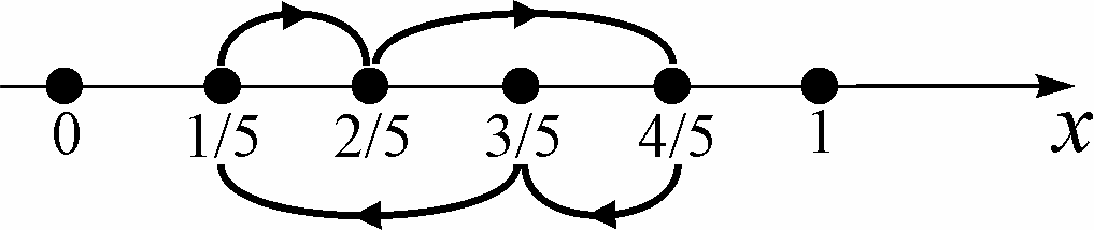
\includegraphics[]{fig/lect1/1}
 	\caption{Полутраектория системы \eqref{eq:1.4} с начальным условием $x(0)=1/5$}
 	\label{fig:1.1}
\end{figure}

% subsubsection динамические_системы_с_дискретным_временем (end)

\subsection{Динамические системы с диссипацией} % (fold)
Рассмотрим динамическую систему \eqref{eq:1.5}  и введем для неё понятие шара диссипации. Говорят, что гладкая поверхность $S=\{\phi(x) = 0 \}$ будет трансверсальной к векторному полю $\vec F (\vec x) $, если скалярное произведение
\begin{equation}
	\qty(\grad \phi(\vec x), \vec F(\vec x)) \neq 0 \qquad \forall \vec x \in S,
\end{equation}
где 
\begin{equation}
	\grad \phi(\vec x) = \qty(\pdv{\phi_1}{x_1},\pdv{\phi_2}{x_2},\dots, \pdv{\phi_m}{x_m})
\end{equation}
Если $S$ топологическая сфера, т.е. граница топологического шара $D$, то шар $D$ называется гаром диссипации, если
\begin{equation}
	\qty(\grad \phi(\vec x), \vec F(\vec x)) < 0 \qquad \forall \vec x \in S,
\end{equation}
Это означает, что векторное поле $\vec F(\vec x)$ на $S$ ориентировано внутрь $D$ (рис. \ref{fig:1.2}). Очевидно, что траектории, входящие в $D$, остаются в нем навсегда. Такие динамические системы называются диссипативными. Наибольшее внимание в нашем курсе будет уделено именно таким динамическим системам, описывающим процессы в физических системах при учете различных потерь. 

\begin{figure}[h!]
	\centering
	
\includegraphics[]{fig/lect1/2}
	\caption{Качественное представление шара диссипации $D$}
	\label{fig:1.2}
\end{figure}


\definition{
\label{def:1.1}
Система \eqref{eq:1.5} называется диссипативной, если существует шар диссипации $D$, такой, что для любой начальной точки $\vec x_0 \in \R^n$: $G^t \vec x_0 \in D$ для некоторого $t>0$.
}

Заметим, что существуют и другие определения диссипативных систем (например, иногда требуют, чтобы $\div \vec F < 0$), но мы будем использовать определение \ref{def:1.1}. 

При исследовании диссипативных систем важную поль играет понятие так называемой поглощающей области.

\definition{\label{def:1.2}
Компактная область $D$ является поглощающей, если 
\begin{equation}
	G^t D \subset \mathrm{Int} D \text{ для } t>0,
\end{equation}}
где $\mathrm{Int} D$ -- внутренняя часть D.

Например, для ДС с дискретным временем вида
\begin{equation}
	\bar x = 3x(1-x)= f(x)
\end{equation}
интервал $[\frac15, \frac45]$ является поглощающей область. Действительно, поскольку 
\begin{equation}
	f\qty(\frac15)=f\qty(\frac45)=\frac{12}{25},\quad f\qty(\frac12)=\frac34,
\end{equation}
то 
\begin{equation}
	f\qty(\qty[\frac15,\frac45])= \qty[\frac{12}{25}, \frac34]\subset \qty(\frac15,\frac45)
\end{equation}
% subsubsection динамические_системы_с_диссипацией (end)
% subsection динамические_системы (end)

\section{Аттракторы} % (fold)

Для систем с диссипацией очень естественно различать переходные процессы и установившиеся процессы или режимы. Базовой чертой установившегося процесса является то, что он «забывает» начальное состояние и не зависит от него. Это означает, что после конечного временного интервала, соответствующего переходному процессу, каждая положительная
полутраектория попадает в малую окрестность некоторого инвариантного множества – <<аттрактора>> (от англ. attract – привлекать, притягивать). Существует несколько определений \href{https://ru.wikipedia.org/wiki/%D0%90%D1%82%D1%82%D1%80%D0%B0%D0%BA%D1%82%D0%BE%D1%80}{аттрактора} (аттрактор Милнора,
статистический аттрактор и др.). Приведем здесь одно из них, которое на наш взгляд наиболее соответствует задачам настоящего курса.
\definition{\label{def:1.3}
Пусть $D$ поглощающая область динамической системы $\qty(G^t, X)$, тогда множество 
\begin{equation}
	A= \bigcap\limits_{t\geq0} G^t D
\end{equation}
называется \textbf{максимальным аттрактором} в $D$.
}
\definition{\label{def:1.4}
Инвариантное множество $A$ является аттрактором, если
существует поглощающая область $D$, для которой $A$ – максимальный аттрактор.
}
Ясно, что максимальный аттрактор зависит от поглощающей области, и может содержать другие аттракторы. Примерами простейших аттракторов являются устойчивые состояния равновесия и неподвижные точки.

% subsection аттракторы (end)

\section{Структурная устойчивость динамических систем} % (fold)
Очевидно, что динамическая система, описывающая поведение любой
реальной системы, должна зависеть от параметров. Рассмотрим, например, систему \eqref{eq:1.5}, зависящую от некоторого набора параметров
\begin{equation}
	\label{eq:1.8}
	\vec {\dot x} = \vec F(\vec x, \vec \mu), \mu \in \R^k,
\end{equation}
где $\mu$ - вектор параметров. Возникает вопрос: нельзя ли обойтись без методов теории колебаний и сделать необходимые нам расчеты динамики системы \eqref{eq:1.8} напрямую, например, численно, используя современные компьютеры и численные методы? Предположим, что мы можем строить приближенно решение системы с любыми начальными условиями. Пусть мы построили какое
– либо решение на некотором временном интервале. Что можно сказать о поведении всей системы, исходя из полученной информации об одном решении? Очевидно – ничего, поскольку в реальных системах начальные условия почти всегда произвольны. Поэтому перебор даже очень большого числа начальных условий не решает полностью задачу, т.к. поведение системы  при оставшихся начальных условиях остается неясным. Кроме того, задачу
усложняет и то, что реальные системы зависят от параметров. Следовательно, используя численное моделирование, мы можем в лучшем случае сказать о  поведении реальной системы только при некоторых значениях параметров и
начальных условий.

Таким образом, для конструирования каких-либо устройств, приборов,
изучения свойств реальных объектов необходимо исследовать не одно какое–либо частное решение системы, а \textbf{целый класс моделей} . Для решения этой
сложной задачи в теории колебаний развивается подход, включающий
следующие базовые положения:
\begin{itemize}
	\item изучать не все траектории системы, а только избранные (в некотором смысле особенные) и находить параметры, при которых такие траектории существуют;
	\item поведение траекторий системы при других значениях параметров изучать, как правило, лишь \textbf{качественно}. 
\end{itemize}

Очевидно, что в динамических системах, описывающих движения
реальных систем, ни один из учитываемых нами факторов не может оставаться абсолютно неизменным во времени. Следовательно, динамические системы, вообще говоря, изменяются вместе с входящими в них параметрами. Однако, если эти изменения достаточно малы, то, как показывает практика, реальная
система как бы не замечает этих изменений, то есть качественные черты ее поведения сохраняются. Поэтому, если мы хотим, чтобы динамическая система отображала эту особенность, нужно придать ей свойство \textbf{грубости}. Именно: при малых изменениях параметров должна оставаться неизменной качественная структура разбиения фазового пространства на траектории. Тем самым выделить класс <<грубых>> динамических систем. Грубость динамической
системы можно трактовать как устойчивость структуры разбиения её фазового пространства на траектории по отношению к малым изменениям динамической
системы. Поэтому грубые динамические системы часто называют структурно устойчивыми.

А.А. Андронов и Л.С. Потрягин (1937 г.) ввели строгое математическое определение грубости динамических систем с двумерным фазовым пространством. Приведем его здесь для системы
\begin{equation}
	\label{eq:1.9}
	\dot x = P(x,y), \quad \dot y = Q(x,y),
\end{equation}
где $P$ и $Q$ -- гладкие функции, а система \eqref{eq:1.9} является диссипативной с шаром диссипации $D$
\definition{\label{def:1.5}
Система \eqref{eq:1.9} называется грубой (структурно устойчивой), если существует такое малое число $\delta>0$m что \textbf{все} динамические системы вида 
\begin{equation}
	\label{eq:1.10}
	\dot x= P(x,y) + p(x,y), \quad \dot y = Q(x,y) + q(x,y),
\end{equation}
в которых аналитические функции $p(x,y)$ и $q(x,y)$ удовлетворяют неравенству
\begin{equation}
	\label{eq:}
	\abs{p(x,y)} + \abs{q(x,y)} +\abs{\pdv{p}{x}} +
	\abs{\pdv{q}{x}}  + \abs{\pdv{p}{y}} + \abs{\pdv{q}{y}} < \delta,
\end{equation}
имеют такую же структуру разбиения $D$ на положительные полутраектории, что и система \eqref{eq:1.9}
}

Совершенно ясно, что не при всяком изменении параметра грубость
динамической системы сохраняется. Можно так поменять параметр, что
произойдет принципиальное изменение фазового портрета. Переход от одной грубой динамической системы к другой происходит через негрубую динамическую систему. Значение параметра, при котором динамическая система является негрубой, называется \textbf{бифуркационным}. Требование грубости для автономных систем второго порядка, являясь естественным с точки зрения приложений, существенно упрощает возможные структуры разбиения фазовой плоскости на траектории. Каждая из этих структур определяется конечным числом особых фазовых траекторий. Что это за траектории речь пойдет ниже в курсе теории колебаний

Заметим, что прямое перенесение, приведенного выше определения
грубости, на случай многомерных (размерность фазового пространства три и выше) динамических систем оказалось невозможным. Было установлено, что существуют многомерные системы, содержащие только неустойчивые траектории, а в пространстве динамических систем существуют целые области
негрубых систем. Поэтому теория грубых многомерных динамических систем строится иначе, чем в двумерном случае. Мы обратимся к этому вопросу позднее.
% subsection структурная_устойчивость_динамических_систем (end)

%\section{Контрольные вопросы и задания} % (fold)
%\begin{enumerate}
	%\item Найти 2- и 3-периодические траектории ДС \eqref{eq:1.7}.
	%\item Показать, что система $\dot x = x- x^3$ является диссипативной.
	%\item Найти поглощающую область для отображения $\bar x= 3.1x(1-x)$
%\end{enumerate}
% subsection контрольные_вопросы_и_задания (end)



% \newpage
% \section{Колебания и волны в цепочке взаимосвязанных тождественных осцилляторов}
% \label{sec:osci_and_wave_in_ordered_struct}
% 	% 08.04.19
% 	%!TEX root = ../lections.tex

Рассмотрим в качестве осциллятора обычный маятник, совершающий малые колебания около нижней точки равновесия. Пусть у нас есть система из связанных осцилляторов (см. рис. \ref{fig:1}): маятники с точками подвеса на расстоянии $a$ друг от друга, связанные пружинками жесткости $\gamma$. 

\begin{figure}[h!]
	\centering
	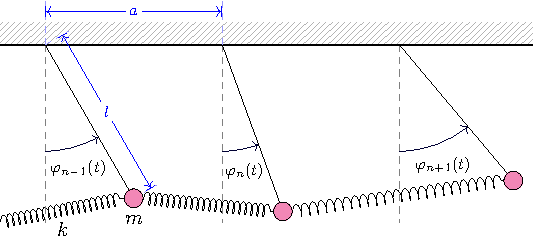
\includegraphics[scale=1.5]{img/osci_and_wave_in_ordered_struct/struct_of_pend}
	\label{fig:fig1}
\end{figure}

Обозначим $n$ -- номер маятника, $\omega_0^2=\frac{g}{l}$ -- собственная частота. Угол отклонения $n$-го маятника $\phi_n$, причем мы рассматриваем случай малых углов.


Состояние маятника зависит не только от времени $t$, но и от номера маятника $n$, то есть $n$ в некотором смысле играет роль пространственной координаты. Запишем уравнение динамики такого маятника:

\begin{equation}
	\ddot{\phi}_n+\omega^2_o \phi_n=\frac{\gamma}{m}\qty[\vphantom{\bigg|}(\phi_{n-1}-\phi_n)+(\phi_{n+1}-\phi_n)].
	\label{eq:1}
\end{equation}

Каждый маятник действует на соседние, причём сила взаимодействия зависит от разности значений углов. Упростим уравнение \eqref{eq:1}:

\begin{equation*}
	\ddot{\phi}_n+\omega^2_o \phi_n=\frac{\gamma}{m}\qty[\vphantom{\bigg|}\phi_{n-1}-2\phi_n+\phi_{n+1}].
\end{equation*}

Часто такую связь называют диффузионной, хотя, конечно, никакого отношения к процессу диффузии она не имеет. В системе нет диссипации, она линейна (нелинейность порождала бы новые частоты). Поэтому решение будем искать в следующем виде:
\begin{equation}
	\phi_n=A e^{i(\omega t-nka)}.
	\label{eq:2}
\end{equation}

Такая форма записи учитывает, что возмущение от маятника к маятнику проходит за некоторое конечное время.
\begin{equation}
	-\omega^2+\omega_0^2=\frac{\gamma}{m}\qty(e^{-ika}-2+e^{ika})
	\quad \Rightarrow \quad
	\omega^2=\omega_0^2-\frac{\gamma}{m}\qty(e^{-ika}-2+e^{ika})
	\label{eq:3}
\end{equation}
Рассмотрим случай  действительного $k$. Тогда
\begin{equation}
	\omega^2=\omega_0^2-\frac{\gamma}{m}(-2+2\cos{ka})=\omega_0^2+\frac{4\gamma}{m}\sin^2{\frac{ka}{2}}.
	\label{eq:4}
\end{equation}
Итак, мы установили, что $\omega$ и $k$ связаны соотношением \eqref{eq:4}. Построим график $\omega(k)$:
\begin{figure}[H]
	\centering
	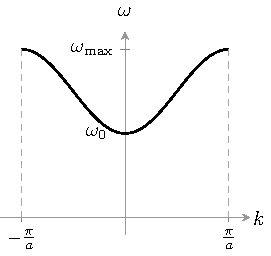
\includegraphics[scale=1.5]{img/osci_and_wave_in_ordered_struct/disp_of_struct}
\end{figure}
Нетрудно получить из уравнения \eqref{eq:4}, что 
\begin{equation*}
	\omega_{\max}=\sqrt{\omega_0^2+\frac{4\gamma}{m}}.
\end{equation*}
Если $\omega_0 < \omega < \omega_{max}$, то каждому $\omega$ соответствуют действительные $k_0$ и $-k_0$. Это означает, что каждой частоте соответствует две гармонические бегущие волны
\begin{equation*}
	\phi_n=A e^{i(\omega t+nk_0a)} 
	\qquad\text{и}\qquad
	\phi_n=A e^{i(\omega t-nk_0a)},
\end{equation*}
где $k_0$ -- волновое число. Поскольку система линейна, любая линейная комбинация решений тоже будет решением. 

Диапазон $\omega_0 < \omega < \omega_{\max}$ называют \textbf{полосой прозрачности} или полосой пропускания. Вне этой полосы решению не отвечают действительные $k$. В этом случае число \textit{$k$ - чисто мнимое} (чисто -- так как нет диссипации в системе) и $k=i\kappa$. Подставив такую связь в \eqref{eq:4}, получим
\begin{equation}
	\omega^2=\omega_0^2-\frac{4\gamma}{m}\sh^2{\frac{\varkappa a}{2}}.
	\label{eq:5}
\end{equation}
Подставляя \eqref{eq:5} в \eqref{eq:2}, получим вид волны в этом случае $\phi_n=A e^{-n\varkappa a} e^{i\omega t}$. Заметим, что при $n\rightarrow \infty$ функция  $\phi_n \rightarrow 0$, то есть в этих областях волна не проходит. 

Если мы находимся в полосе прозрачности, то $v_\text{фаз}=v_\text{фаз}(k), v_\text{фаз}=v_\text{фаз}(\omega)$. Если фазовая скорость зависит от частоты или волнового числа, то среда диспергирующая, а \eqref{eq:4} - дисперсионное соотношение. 

Дисперсия возникает из-за наличия собственных пространственных и временных масштабов : $a$ и $\omega_0$. У каждой компоненты волнового пакета будет своя фазовая скорость, возникнет его деформация. Именно наличием собственных масштабов объясняется то, что в одних случаях система пропускает волну, а в других нет.





\subsection{Предельный переход от цепочной структуры к среде}
Введём пространственную координату $x$ вдоль балки, на которой расположены точки подвеса. Сделаем замену, считая, что $\phi_n$ зависит от двух переменных:
\begin{equation*}
	\phi_n(t) \rightarrow \phi(x,t).
\end{equation*}
Считая $a$ малым, разложим $\phi_{n\pm 1}$ в ряд Тейлора по степеням $a$:
\begin{gather}
	\phi_{n+1}(t) \rightarrow \phi(x+a,t)=\phi(x,t)+\pdv{\phi}{x}a +\frac12 \pdv[2]{\phi}{x}a^2+\ldots,\\\nonumber
	\phi_{n-1}(t) \rightarrow \phi(x-a,t)=\phi(x,t)-\pdv{\phi}{x}a +\frac12 \pdv[2]{\phi}{x}a^2+\ldots
	\label{eq:6}
\end{gather}
Полученные разложеня до второго порядка подставим в \eqref{eq:1}:
\begin{gather*}
	\pdv[2]{\phi}{t} + \omega_0^2 \phi=\frac{\gamma}{m}a^2 \pdv[2]{\phi}{x}.
\end{gather*}
Обозначим $\frac{\gamma}{m}a^2 = v^2$, тогда уравнение  примет вид, известный как \textbf{уравнение Клейна-Гордона}:
\begin{equation}
	\pdv[2]{\phi}{t}-v^2\pdv[2]{\phi}{x}+\omega_0^2\phi=0.
	\label{eq:7}
\end{equation}
Уравнение \eqref{eq:7} не что иное, как уравнение в частных производных. Когда мы можем использовать \eqref{eq:7} вместо \eqref{eq:1}? Вспомним, что мы предполагали при решении задачи:
\begin{enumerate}
	\item Угол $\phi_n$, определенный в точке, определен и между дискретными точками подвеса;
	\item Отброшены величины третьего порядка;
	\item Расстояние между точками подвеса $a$ -- мало
\end{enumerate}

Построим дисперсионную характеристику для \eqref{eq:7}. Для этого подставим решение в виде бегущей волны в \eqref{eq:7}:
\begin{gather*}
	\phi(x,t)=Ae^{i(\omega t + kx)} \quad \Rightarrow \quad -\omega^2-k^2v^2+\omega_0^2=0,
\end{gather*}
\begin{equation}
	\omega^2 = \omega_0^2 + k^2v^2.
	\label{eq:8}
\end{equation}
\begin{figure}[H]
	\centering
	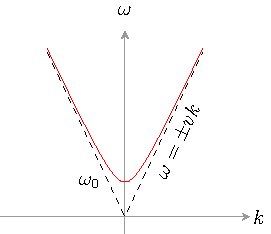
\includegraphics[scale=1.5]{img/osci_and_wave_in_ordered_struct/disp_of_cont}
\end{figure}
Нетрудно получить, что график имеет две асимптоты $\omega=\pm vk$. 

\paragraph{Условие совпадения дисперсионных соотношений. } При $\lambda\gg a$ или $ka\ll$ -- это условие длинноволновой зоны -- можно от соотношения \eqref{eq:4} перейти к \eqref{eq:8}. В этом случае пространственный масштаб не сказывается и мы им пренебрегаем. 

Если  $\omega_0 \rightarrow 0$, то из \eqref{eq:8} следует, что $\omega^2=k^2v^2$. В этом случае система не обладает дисперсией:

\begin{figure}[H]
	\centering
	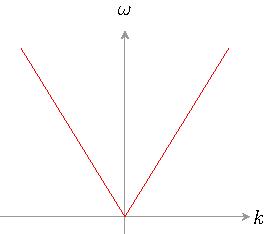
\includegraphics[scale=1.5]{img/osci_and_wave_in_ordered_struct/no_disp} 
\end{figure}

Дисперсионная характеристика проявляется в областях прозрачности или непрозрачности и зависимости $v_\text{фаз}$ от $k$ или $\omega$.

% Получили, шарики плотно друг к другу и покоятся.

Переход от цепочки к среде называется длинноволновым переходом: при нем теряется дискретность системы.

\subsection{Составление дисперсионного уравнения для произвольной линейной системы}

Рассмотрим многомерную систему
\begin{equation}
	A\pdv{\vec{U}}{t}+B\pdv{\vec{U}}{x}+C\vec{U}=0.
	\label{eq:9}
\end{equation}

A, B, C - $n\times n$ - матрицы; $\vec{U}(x,t)$ описывает состояние системы.

\begin{equation}
	\vec{U}=\vec{\phi} e^{i(\omega t - kx)}.
	\label{eq:10}
\end{equation}

\begin{equation*}
	\vec\phi=
	\begin{pmatrix}
		\phi_1 \\
		\phi_2 \\
		\phi_3 \\
		\vdots \\
		\phi_n \\
	\end{pmatrix}
	,
\end{equation*}

\begin{equation*}
	Ai\omega\vec\phi-iBk\vec\phi+C\vec\phi=0,
\end{equation*}
\begin{equation}
	(A\omega-Bk-iC)\vec\phi i=0.
	\label{eq:11}
\end{equation}

\eqref{eq:11} представляет собой систему линейных однородных уравнений относительно компонент вектора $\vec\phi$. Она имеет решение, если ее детерминант
\begin{equation}
	det(A\omega-Bk-iC)=0.
	\label{eq:12}
\end{equation}

для краткости обозначают $D(\omega,k)=0$. он связывает $\omega$ и k, т.е. задает дисперсионную характеристику. Следовательно, для $\forall k$ дисперсионное соотношение определяют n значений $\omega$: $\omega_1(k), \dots, \omega_n(k)$. Каждой паре k, $\omega_s(k)$ отвечает некоторый вектор, определяемый \eqref{eq:11}. При этом решением будут не только $k, \omega, \vec\phi$, но и $k^*, \omega^*, \vec\phi^*$. Можно построить действительное решение:
\begin{equation}
	\vec{U}(x,t)=\vec\phi e^{i(\omega t-kx)}+\vec\phi^* e^{-i(\omega^* t-k^*x)}.
	\label{eq:13}
\end{equation}

\eqref{eq:13} задает гармоническую волну, если $k, \omega$ действительные. Если же $k, \omega$ комплексные, то \eqref{eq:13} задает нарастающее или затухающее колебание. При этом общее решение может выть записано в виде 
\begin{equation*}
	\vec{U}(x,t)=\sum_{s=1}^{n} \phi^{(s)}e^{i(\omega_s(k)t-kx)} + \text{к.с}.
\end{equation*}

Как только будут учтены граничные условия, получится аналог характеристического уравнения.

\subsection{Влияние граничных условий}
Предположим, маятники были свернуты в кольцо, следовательно, должно уложиться целое число полуволн: 

\begin{gather*}
	n=1,\dots,N;~~\phi_{n-1}-2\phi_n+\phi_{n+1}; \\
	k=\frac{2\pi n}{l};~~\phi_{N+1}=\phi_1;~~k=k_n.
\end{gather*}	

Примером распределенной системы может служить струна длины l, концы которой закреплены:
\begin{figure}[H]
	\centering
	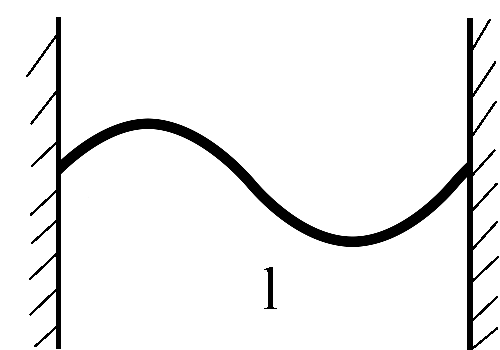
\includegraphics[width=0.5\linewidth]{fig/fig5.pdf}   
\end{figure}
\begin{gather*}
	U(x,t), \\ U(0,t)=u(l,t)=0, \\ U(x,t)=\phi_1 e^{i(\omega t-kx)}+\phi_2 e^{i(\omega t+kx)}, \\
	\begin{cases}
		\phi_1 e^{i\omega t}+\phi_2 e^{i\omega t}=0 \\
		\phi_1 e^{i\omega t}+\phi_2 e^{i\omega t+ikl}=0
	\end{cases}
	\\ \phi_1=-\phi_2,~~ \sin{kl}=0,~~ k=\frac{\pi n}{l}=k_n
\end{gather*}

\begin{equation}
	\begin{cases}
		D(\omega,k)=0 \\
		k=k_n
	\end{cases}
	\label{eq:14}
\end{equation}

Отсюда следует, что $\omega=omega_n$. Если среда без дисперсии, то спектры волновых чисел и волновых частот будут эквидистантными. 

\subsection{Устойчивость состояний равновесия нелинейных распределенных систем}
Простейшим типом решений распределенных систем являются такие состояния, которые не меняются ни во времени, ни в пространстве: $U(x,t); U=U_o=const$.
\begin{equation}
	\pdv{U}{t}=f(U)+D\pdv[2]{U}{x},
	\label{eq:15}
\end{equation}
где $f(U)$ - нелинейная функция. Пусть, кубическая. Если убрать D. то уравнение будет описывать динамику точки в среде.
\begin{figure}[H]
	\centering
	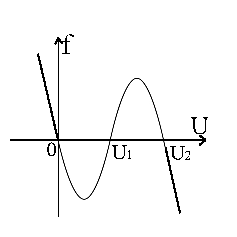
\includegraphics[width=0.5\linewidth]{fig/fig6.pdf}   
\end{figure}

Три точки, где $f(U)=0$. В системе могут быть стационарные решения (не зависящие от времени) - это другой тип решения. Будем рассматривать их решение в классе гармонических функций. 
\begin{equation*}
	\xi(x,t) \sim e^{pt+ikx}
\end{equation*}

Линеаризуем \eqref{eq:15} на состояниях равновесия:
\begin{equation*}
	U=U^*+\xi(x,t),
\end{equation*}
\begin{equation}
	\pdv{\xi}{t}=D\pdv[2]{\xi}{x}+f'(U^*)\xi(x,t).
	\label{eq:16}
\end{equation}
\begin{gather*}
	f(U^*+\xi(x,t))\approx f(U^*)+f'(U^*)\cdot\xi(x,t), \\ \xi(x,t)=A e^{pt+ikx} \\
	p =-Dk^2+f'(U^*), \\ U=0,~~U=U_2,~~f'(U^*)<0.
\end{gather*}

Для каждого А.
\begin{figure}[H]
	\centering
	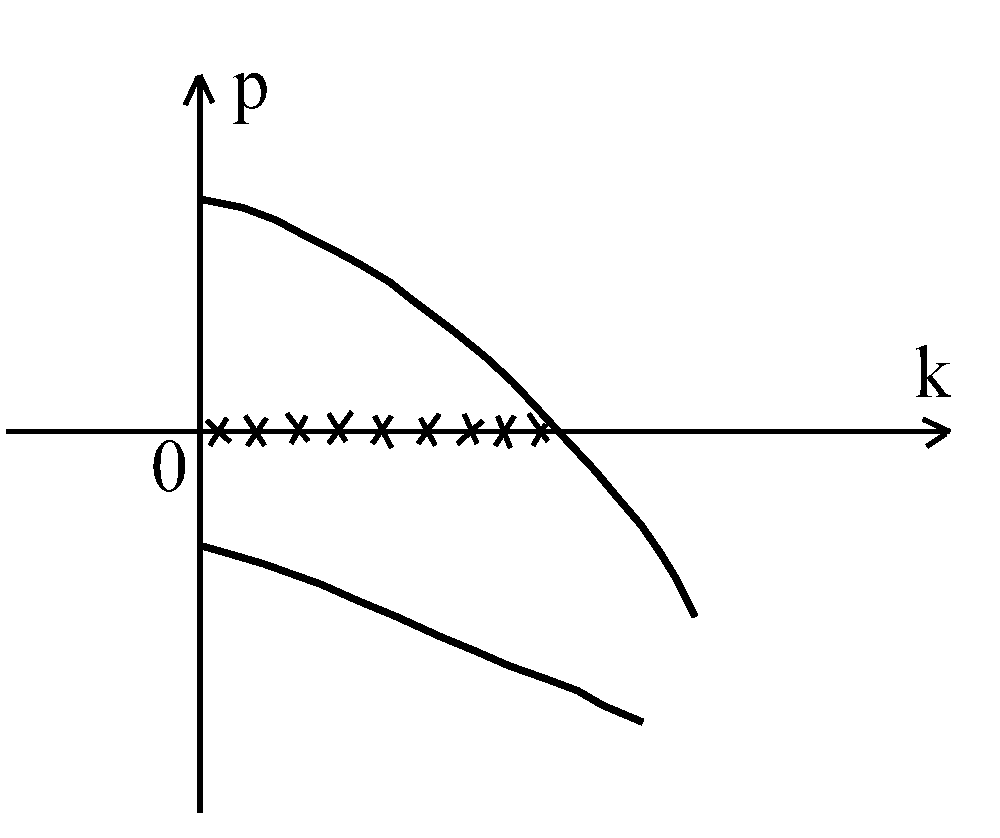
\includegraphics[width=0.5\linewidth]{fig/fig7.pdf}   
\end{figure}

Все решения такого вида затухают, следовательно, $U=0, U=U_2$ устойчивые, а $U_1$ - неустойчивое в классе возмущений $\xi(x,t)=A e^{pt+ikx}$.

В частности, \eqref{eq:15}, описывает распространение пламени по бикфордовому (огнепроводному) шнуру. Волна превращает вещество из несгоревшего материала в сгоревшее.


% \newpage
% \section{Диффузионная неустойчивость. Структура Тьюринга}
% \label{sec:diffusion_instability}
% 	% 15.04.19
% 	Многие биологические объекты обладают периодической структурой. Например, зебра, дождевой червь, сороконожка. Однако известно, что изначально, при появлении, они однородны. Рассмотрим одномерный случай структур.

Тьюринг предположил, что существуют два вещества. Одно из них - $U(x,t)$ - стимулирует рост клеток. Его назвали активатором. Другое - $V(x,t)$ - замедляет рост. Это ингибитор. Следующим предположением было наличие некоторых химических реакций и присутствие диффузии. Фактически, Тьюринг записал уравнение реакции диффузии. 
\begin{equation}
\begin{cases}
		\pdv{U}{t}=f(U,V)+D_1 \pdv[2]{U}{x} \\
		\pdv{V}{t}=g(U,V)+D_2 \pdv[2]{V}{x},
	\end{cases}	\
	\label{eq:17}
\end{equation}
где $f,g$  - это некоторые нелинейные функции.

Эта система двухкомпонентная, произвольная координата одна. Предположим, \eqref{eq:17} имеет состояние равновесия, т.е. существует решение системы
\begin{equation}
\begin{cases}
		f(U,V)=0 \\
		g(U,V)=0.
	\end{cases}	\
	\label{eq:18}
\end{equation}
$U=U_0, V=V_0$.

Исследуем на устойчивость. Положим,
\begin{gather*}
	U=U_0+\xi(x,t) \\
	V=V_0+\eta(x,t).
\end{gather*}

Линеаризуем (оставляем только линейную часть):
\begin{equation}
	\begin{cases}
		\pdv{\xi}{t}=f'_u(U_0, V_0)\xi(x,t)+f'_v(U_0, V_0)\eta(x,t)+D_1 \pdv[2]{\xi(x,t)}{x} \\
		\pdv{\eta}{t}=g'_u(U_0, V_0)\xi(x,t)+g'_v(U_0, V_0)\eta(x,t)+D_2 \pdv[2]{\eta(x,t)}{x}.
	\end{cases}	
	\label{eq:19}
\end{equation}

Получили уравнения в частных производных. Будем искать решение в виде:
\begin{equation}
	\xi(x,t)=A e^{pt+ikx};~~\eta(x,t)=B e^{pt+ikx}.
	\label{eq:20}
\end{equation}

Подставляя эти решения и учитывая, что $f'$ и $g'$ - это производные в точке, т.е. константы, получим:
\begin{equation}
	\begin{cases}
		\pdv{\xi}{t}=a\xi+b\eta+D_1 \pdv[2]{\xi}{x} \\
		\pdv{\eta}{t}=c\xi+d\eta+D_2 \pdv[2]{\eta}{x},
	\end{cases}	
	\label{eq:21}
\end{equation}
где
\begin{gather*}
	a=f'_u(U_0, V_0),~~b=f'_v(U_0, V_0),~~c=g'_u(U_0, V_0),~~d=g'_v(U_0, V_0).
\end{gather*}

\begin{equation}
	\begin{cases}
		Ap=aA+bB-k^2 D_1A \\
		Bp=cA+dB-k^2 D_2A,
	\end{cases}	
	\label{eq:22}
\end{equation}

\eqref{eq:17} представляет собой систему линейных однородных уравнений относительно констант А,В. Она имеет нетривиальное решение, если ее определитель не равен нулю. Раскрывая определитель, получим характеристическое уравнение для p:
\begin{equation}
	p^2+(D_2k^2+D_1k^2-a-d)p+(D_1k^2-a)(D_2k^2-d)-bc=0.
	\label{eq:23}
\end{equation}

Предположим, что в начальный момент $D_1=D_2=0$, тогда
\begin{equation}
	p^2-(a+d)p+ad-bc=0.
	\label{eq:24}
\end{equation}

Сначала структуры у животных нет, следовательно, без диффузии имеем устойчивое равновесие. Запишем условие для этого:
\begin{gather*}
	\Delta_o=ad-bc>0, \\ \sigma_0=a+d<0,
\end{gather*}
тогда состояние равновесия будет устойчивым. 

\begin{figure}[H]
	\centering
	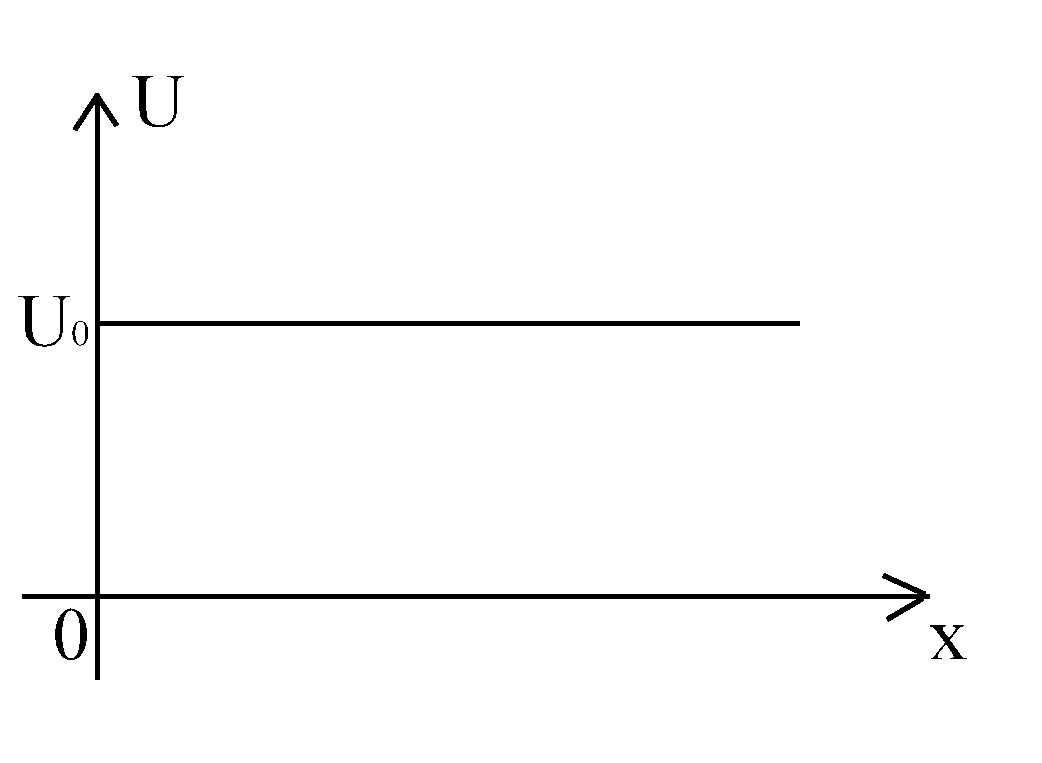
\includegraphics[width=0.5\linewidth]{fig/fig8.pdf}   
\end{figure}

По оси х U(активатор) и V(ингибитор) постоянны. 

Пусть теперь $D_1, D_2 \neq 0$. В этом случае \eqref{eq:24} после преобразований примет вид:
\begin{equation*}
	p^2-\sigma p+\Delta=0,
\end{equation*}
где
\begin{gather*}
	\Delta=a+d-(D_1+D_2)k^2=\sigma_0-(D_1+D_2)k^2, \\ \sigma=ad-bc-(aD_2+dD_1)k^2+D_1D_2k^4=\Delta_0-(aD_2+dD_1)k^2+D_1D_2k^4.
\end{gather*}

$Re\{p\}$ зависит от k. Анализ показывает:
\begin{figure}[H]
	\centering
	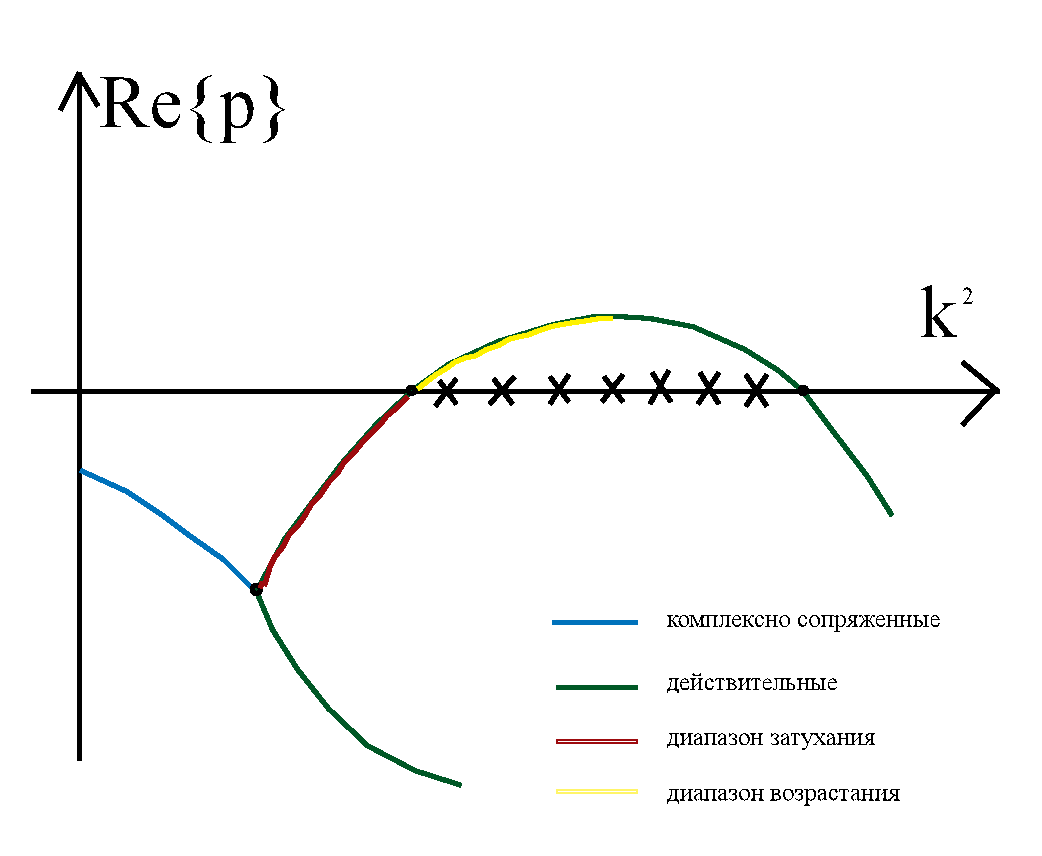
\includegraphics[width=0.5\linewidth]{fig/fig9.pdf}   
\end{figure}

Есть диапазон, где произошла потеря устойчивости состояния равновесия за счет действия диффузии. Это называется диффузионной неустойчивостью. Возникает аналог бифуркации Андронова-Хопфа. В диапазоне затухания все моды затухают, а возрастания - возрастают. Возникает периодическое по пространственной координате решение. Кроме того, оно пространственно неоднородное.  
\begin{figure}[H]
	\centering
	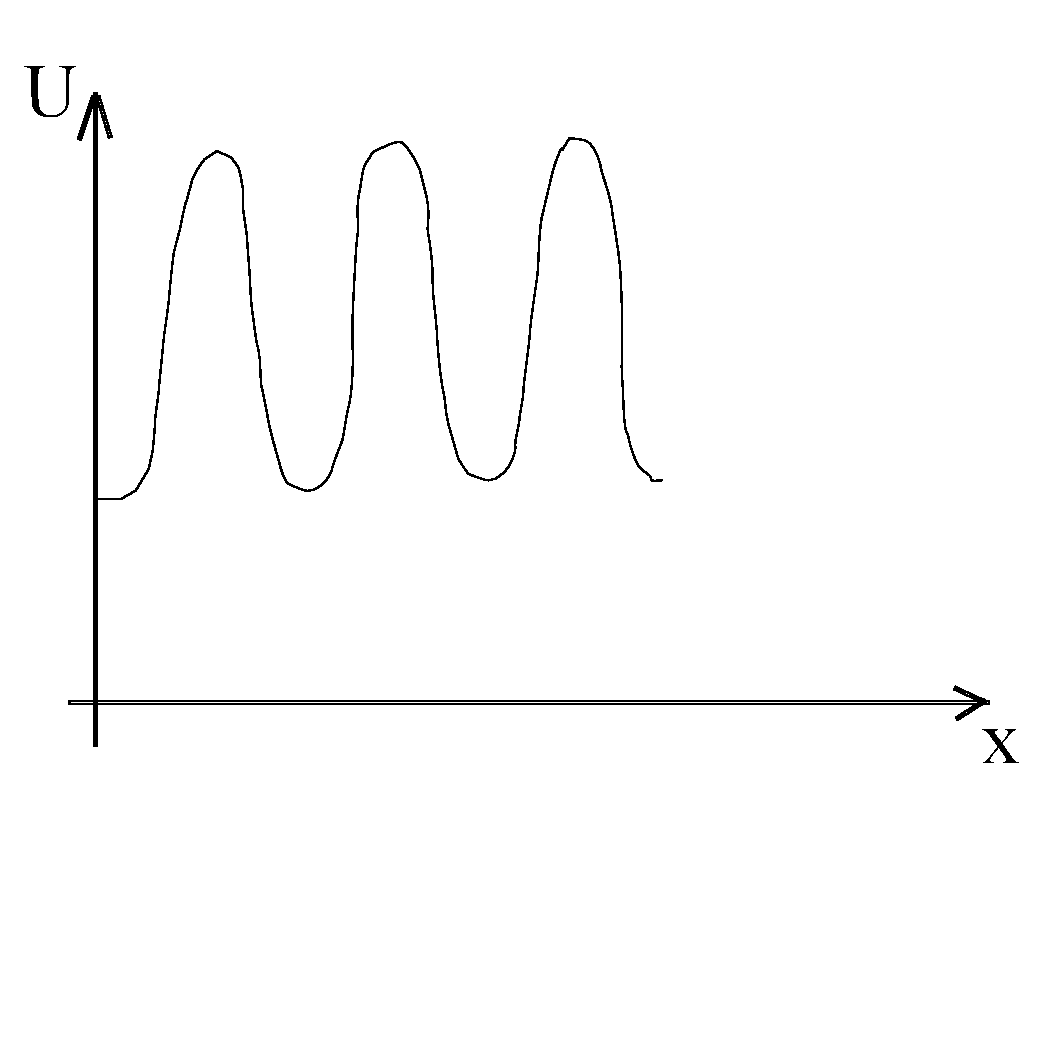
\includegraphics[width=0.5\linewidth]{fig/fig10.pdf}   
\end{figure}

Динамическая структура, обладающая свойством структурной устойчивости, иногда называется диссипативной структурой. Возникает за счет баланса. 

\subsection{Простые волны. Образование разрывов.}
Рассмотрим равномерную среду, свойства которой описывает скалярная функция $U(x,t)$. Среда линейная, без дисперсия. В таких средах возможно существование волновых движений, при этом все переменные описываются одинаковыми уравнениями:
\begin{equation}
	\pdv{U_j}{t}+V\pdv{U_j}{x}=0.
	\label{eq:25}
\end{equation}

В среде нет собственных масштабов и нелинейностей. V-const. В этой среде возможно существование так называемых римановых волн. 
\begin{equation}
	U_j=\phi(x-Vt),
	\label{eq:26}
\end{equation}
где $\phi$ - произвольная, обязательно дифференцируемая, функция.

Введем бегущую координату:
\begin{gather*}
	\xi=x-Vt, \\ \dv{\phi}{\xi} \pdv{\xi}{t}+V\dv{\phi}{\xi} \pdv{\xi}{x}=0, \\ -V\dv{\phi}{\xi}+V\dv{\phi}{\xi} \equiv 0.
\end{gather*}

\eqref{eq:26} является решением такой системы. 

Теперь рассмотрим нелинейную среду (но все еще без дисперсии). В таких средах могут существовать волны, которые обладают следующим свойством: переменные связаны алгебраически (если есть $U_1$ и $U_2$, то $U_3$ всегда можно пересчитать).

Рассмотрим пример: волны на мелкой воде. Гравитационные волны вдоль оси x.
\begin{figure}[H]
	\centering
	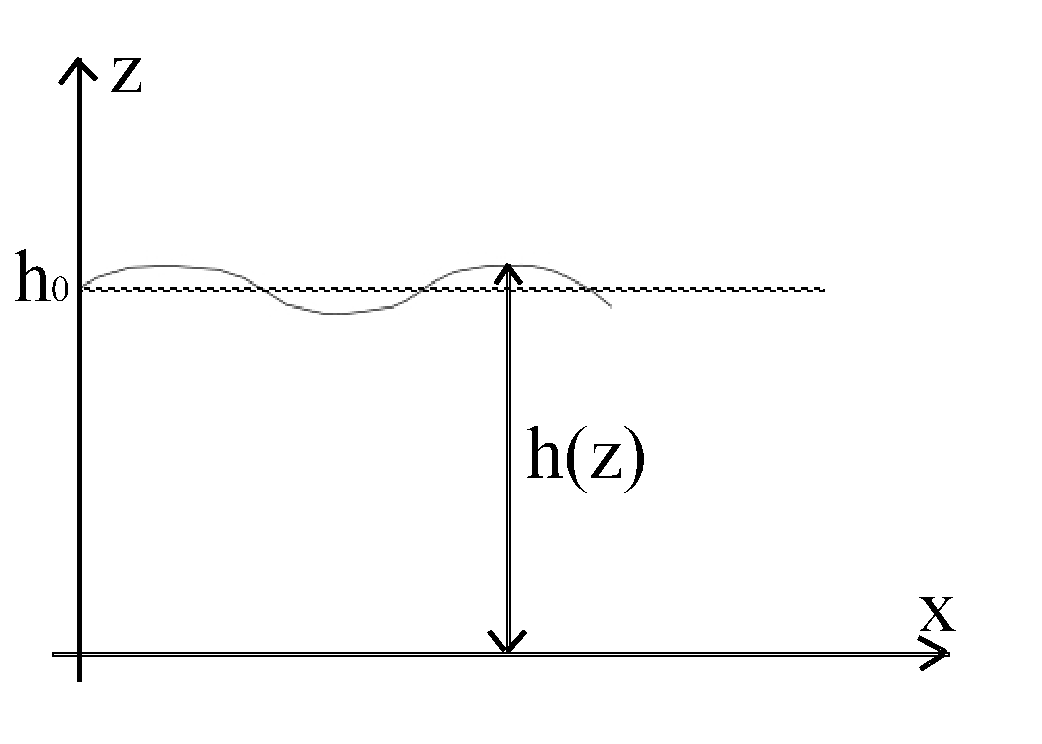
\includegraphics[width=0.4\linewidth]{fig/fig11.pdf}   
\end{figure}
$\lambda \gg h_0$

Состояние жидкости описывается: V - скоростью волны, h - профилем. Поскольку волны длинные, считаем, что $V\neq V(z)$.

Используем уравнение Эйлера: 
\begin{gather*}
	\pdv{V}{t}+V\pdv{V}{x}+\frac1{\rho}\pdv{\rho}{x}=0, \\ \rho=const, p-\text{среднее по высоте}, \\ \frac1{\rho}\pdv{\rho}{x}=g\pdv{h}{x}.
\end{gather*}

Давление больше там, где выше жидкость.
\begin{equation}
	\pdv{V}{t}+V\pdv{V}{x}+g\pdv{h}{x}=0.
	\label{eq:27}
\end{equation}

Добавим уравнение непрерывности:
\begin{gather*}
	\pdv{p}{t}+\pdv{(Vh)}{x}=0. 
\end{gather*}

Скорость изменения высоты слоя связана с разностью потока через x и dx
\begin{equation}
	\pdv{h}{t}+V\pdv{h}{x}+h\pdv{V}{x}=0.
	\label{eq:28}
\end{equation}

Предположим, h и V не являются независимыми переменными и $h=h(V)$.

Из уравнения \eqref{eq:27}: 
\begin{gather*}
	\pdv{h}{x}=\dv{h}{V}\pdv{V}{x}, \\ \pdv{V}{t}+V\pdv{V}{x}+g\pdv{h}{x} = 0 ~(*).
\end{gather*}

Из уравнения \eqref{eq:28}:
\begin{gather*}
	\dv{h}{V}\pdv{V}{t}+V\dv{h}{V}\pdv{V}{x}+h(V)\pdv{V}{x} = 0, \\ \pdv{V}{t}+V\pdv{V}{x}+\frac{h(V)}{\dv{h}{V}}\pdv{h}{x} = 0 ~(**).
\end{gather*}

(*) и (**) должны совпадать, т.к описывают одну и ту же величину. 
\begin{equation*}
	g\dv{h}{V}=\frac{h}{\dv{h}{V}}~ \text{или} ~(\dv{h}{V})^2=\frac{h}{g} - \text{уравнение для нахождения h}.
\end{equation*}

\begin{gather*}
	\dv{h}{V}=\pm \sqrt{\frac{h(V)}{g}}, \\ \pdv{V}{t}+V\pdv{V}{x}\pm \sqrt{h(V)g} \pdv{V}{x} = 0.
\end{gather*}
\begin{equation}
	\pdv{V}{t}+(V\pm \sqrt{h(V)g})\pdv{V}{x} = 0
	\label{eq:29}
\end{equation}
- уравнение простой волны, которое в общем виде выглядит:
\begin{equation}
	\pdv{U}{t}+V(U)\pdv{U}{x} = 0
	\label{eq:30}
\end{equation}

Это уравнение справедливо не только на мелкой воде. Здесь $V$ - это функция среды.

Будем искать решение в виде:
\begin{equation}
	U = \phi(x-V(U)t),
	\label{eq:31}
\end{equation}
\begin{gather*}
	\xi=x-V(U)t.
\end{gather*}

Убедимся, что \eqref{eq:30} - решение:
\begin{gather*}
	\pdv{U}{t}=\dv{\phi}{\xi}\pdv{\xi}{t}=\dv{\phi}{\xi}\qty(-V(U)-t\dv{V}{U}\pdv{U}{t}), \\ \pdv{U}{t}\qty(1+\dv{\phi}{\xi}\dv{V}{U}t)=-V(U)\dv{\phi}{\xi},
\end{gather*}
\begin{equation}
	\pdv{U}{t}=-V(U)\dv{\phi}{\xi} \frac{1}{(1+\dv{\phi}{\xi}\dv{V}{U}t)}
	\label{eq:32}
\end{equation}
\begin{gather*}
	\pdv{U}{x}=\dv{\phi}{\xi} \frac{1}{(1+\dv{\phi}{\xi}\dv{V}{U}t)}
\end{gather*}

Для определенности:
\begin{figure}[H]
	\centering
	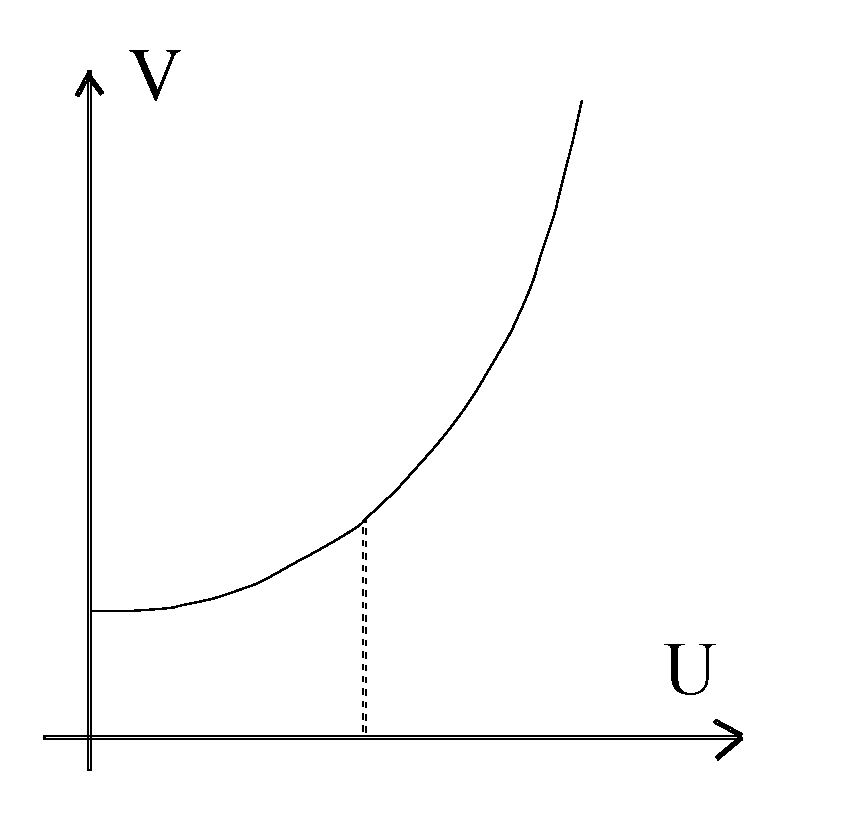
\includegraphics[width=0.4\linewidth]{fig/fig12.pdf}   
\end{figure}

У максимального значения U скорость наибольшая. Задается профиль $\phi$ при $t=0$:
\begin{figure}[H]
	\centering
	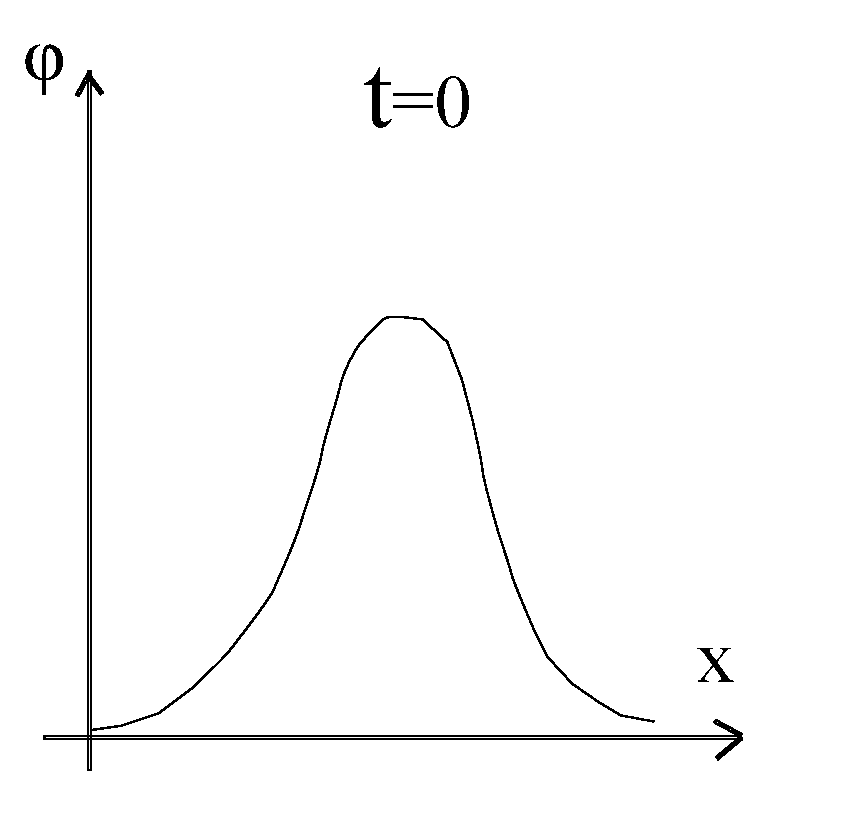
\includegraphics[width=0.4\linewidth]{fig/fig13.pdf}   
\end{figure}
или при $x=0$:
\begin{figure}[H]
	\centering
	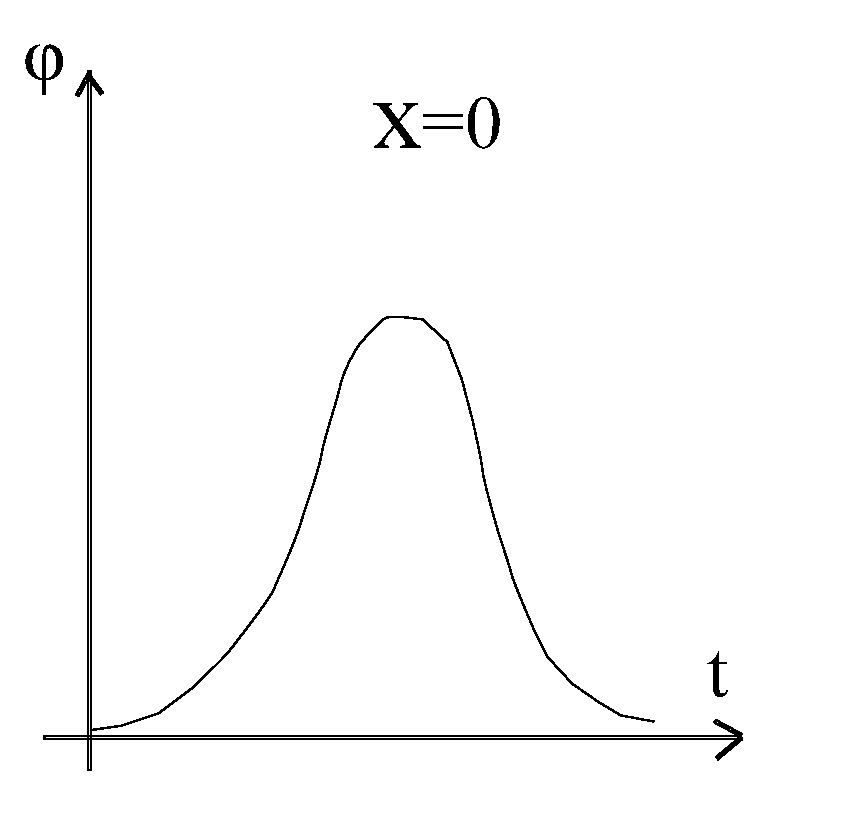
\includegraphics[width=0.4\linewidth]{fig/fig14.pdf}   
\end{figure}

Во время распространения, верх волны обгонит, произойдет укручение фронта, волна деформируется. 
\begin{figure}[H]
	\centering
	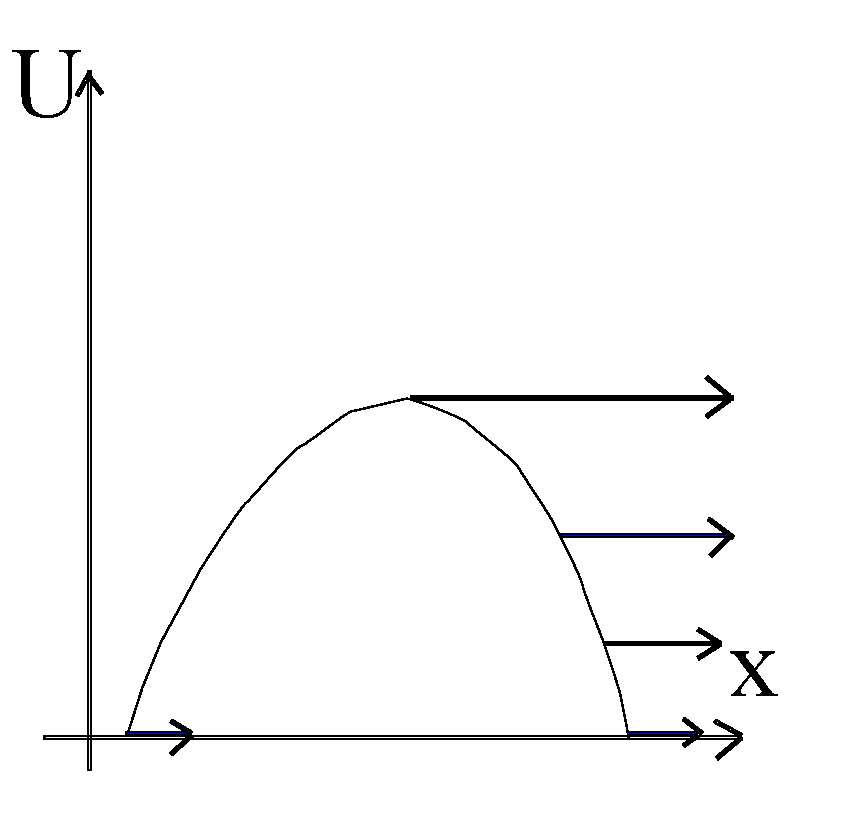
\includegraphics[width=0.4\linewidth]{fig/fig15.pdf}   
\end{figure}
\begin{figure}[H]
	\centering
	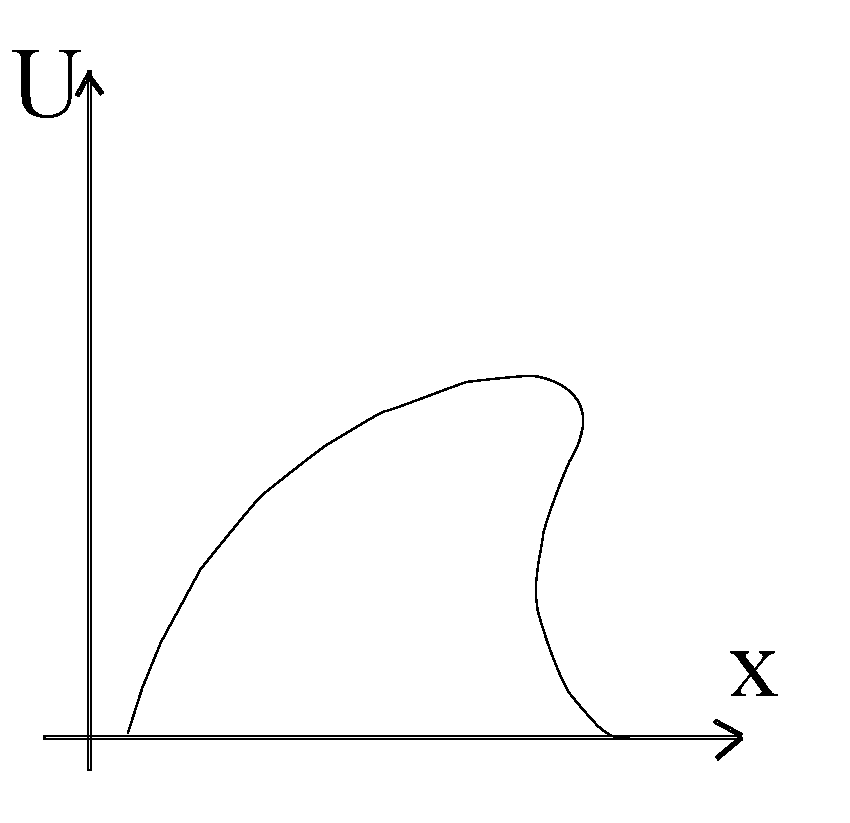
\includegraphics[width=0.4\linewidth]{fig/fig16.pdf}   
\end{figure}
\begin{figure}[H]
	\centering
	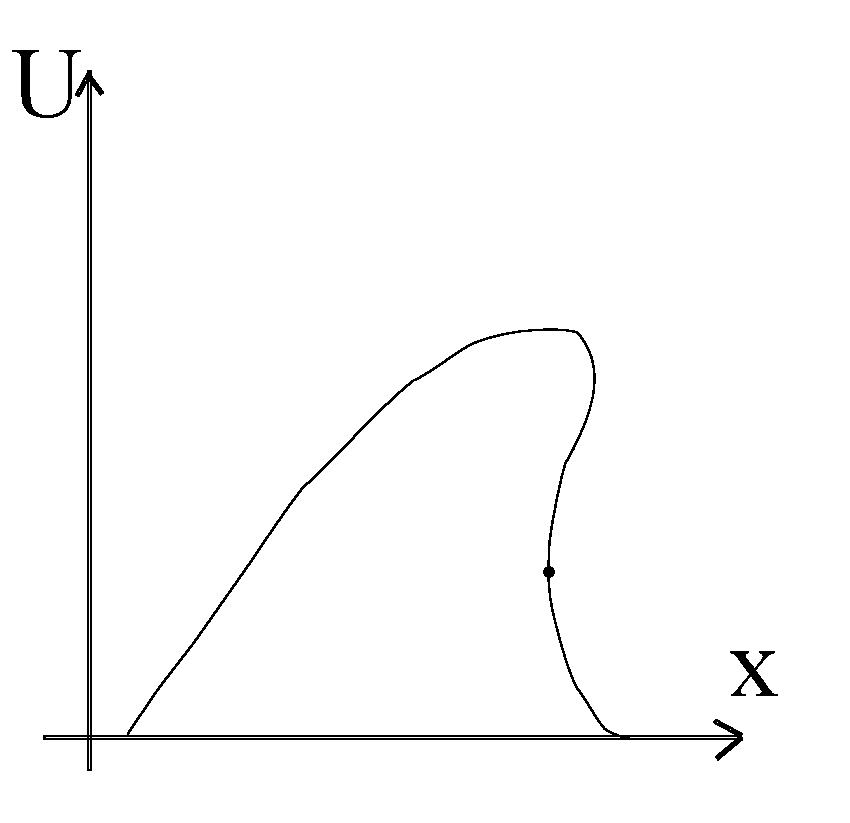
\includegraphics[width=0.4\linewidth]{fig/fig17.pdf}   
\end{figure}

Появится точка, где производные $\pdv{U}{t}, \pdv{U}{x} \rightarrow \infty $. Образуется бесконечный градиент и разрыв, который характеризуется состоянием $U^*, t^*, x^*$, его описание в рамках простой волны несправедливо. Вторые производные тоже обращаются в бесконечность, и точки эти можно найти.



% \newpage
% \section{Солитоны в уравнении Кортевега -- де Вриза}
% \label{ssec:soliton}


% %!TEX root = ../lections.tex
Экспериментально получить явление, увиденное Расселом, можно следующим образом. Берется узкий, достаточно длинный бассейн, разделённый перегородкой:  
\begin{figure}[H]
	\centering
	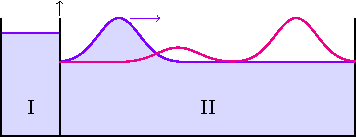
\includegraphics[scale=1.5]{img/soliton/pool}
\end{figure}
Подбирается соотношение масс воды в емкостях, при этом в части I уровень всегда должен быть выше. Резко поднимают задвижку, и, в зависимости от соотношения масс воды, могут побежать разные волны: разное количество холмов. 

В 1985 году Кортевег и де Вриз написали уравнения, описывающие явление, обнаруженное Расселом, и нашли форму волнового движения. Они рассматривали мелкий канал  со средней глубиной $l$, уровень воды $l+\eta(x,t)$, и получили следующее уравнение: 
\begin{equation*}
	\pdv{\eta}{t}=\frac32 \sqrt{\frac{g}{l}}\pdv{}{x}\qty(\frac32 \alpha \eta+\frac12 \eta^2+\frac13 \sigma \pdv[2]{\eta}{x}),
\end{equation*}
где $\sigma=\frac{l^3}{3}-\frac{Tl}{\rho g}$, $\alpha$ -- произвольная константа, $T$ -- коэффициент поверхностного натяжения, $\rho$ -- плотность жидкости.

В упрощённом виде это уравнение можно записать так:
\begin{equation}
	\pdv{u}{t}+u\pdv{u}{x}+\beta \pdv[3]{u}{x}=0.
	\label{eq:s3:1}
\end{equation}
Здесь $\beta$ -- некоторая константа, а последнее слагаемое характеризует дисперсию. Это уравнение простой волны, дополненное дисперсией. \textbf{Задание к  экзамену: построить дисперсионную характеристику}. 

\paragraph{Что дает дисперсия? } Рассмотрим квадратично-нелинейную среду без дисперсии.
Запустим в неё волну $e^{i(\omega_o t+kx)}$. Квадратичная среда порождает новые частоты: $\omega_0$ порождает $2\omega_0$. Если нет дисперсии, то нет пространственных масштабов, $2\omega_0$ порождает $3\omega_0$ и так далее, лавинным образом, спектр стремится в бесконечность. 
% \begin{figure}[H]
% 	\centering
% 	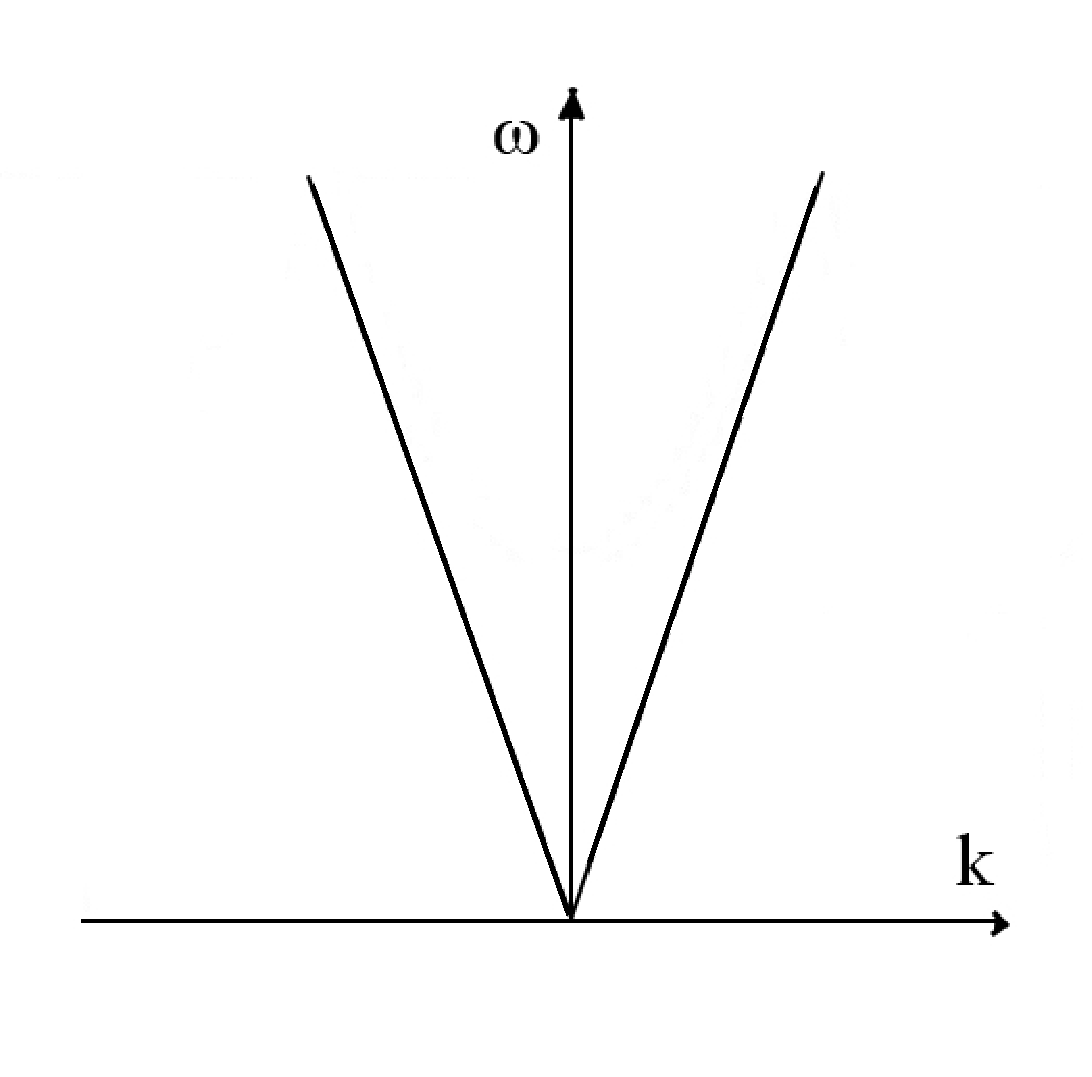
\includegraphics[width=0.4\linewidth]{fig/fig4.pdf}   
% \end{figure}

Слагаемое $\beta\pdv[3]{u}{x}$ даёт высокочастотную дисперсию, ограничивает ВЧ-спектр, стабилизирует решение и порождает солитон.
% Теперь включим дисперсию (в данном случае - высокочастотную). Она ограничивает частотный рост и стабилизирует волну. 

\paragraph{Решение задачи о солитоне. } Будем искать решение уравнения \eqref{eq:s3:1} в виде $u=u(x-Vt)=u(\xi)$, где $V=\const$:
\begin{equation}
	-\pdv{u}{\xi}+u\pdv{u}{\xi}+\beta \pdv[3]{u}{\xi}=0.
	\label{eq:s3:2}
\end{equation}
Один раз интегрируя, получим
\begin{equation}
	\beta \pdv[2]{u}{\xi}+\frac{u^2}{2}-Vu=0.
	\label{eq:s3:3}
\end{equation}
Это уравнение нелинейного осциллятора. Для простоты константу интегрирования приравняли  к нулю, что дает уровень, откуда изменяется $u(x,t)$. Запишем уравнение в виде системы
\begin{equation}
	\left\{\begin{aligned}
		&\dot{u}=y \\
		\beta &\dot{y} =Vu-\frac{u^2}{2}.		
	\end{aligned}\right.
	\label{eq:s3:4}
\end{equation}
% Получили систему для нелинейного осциллятора.
Можем найти потенциальную энергию, проинтегрировав правую часть второго уравнения системы \eqref{eq:s3:4}:
\begin{gather*}
	\beta \frac{y^2}{2}+E_{\text{п}} = \const
	\quad \Rightarrow \quad
	 E_{\text{п}} = \frac{u^3}{6}-V\frac{u^2}{2}
\end{gather*}
\begin{figure}[H]
	\centering
	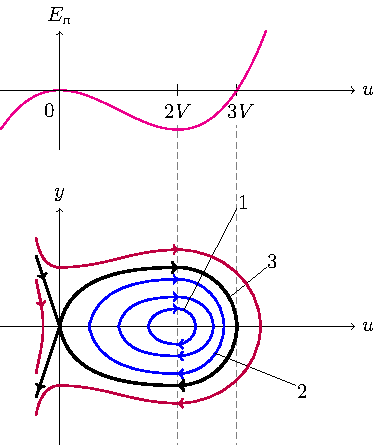
\includegraphics[scale=1.5]{img/soliton/phase_port_nonlin_osci}
	\caption{Фазовый портрет нелинейного осциллятора \eqref{eq:s3:4}}
	\label{fig:phase_port}
\end{figure}

% Фазовый портрет:
% \begin{figure}[H]
% 	\centering
% 	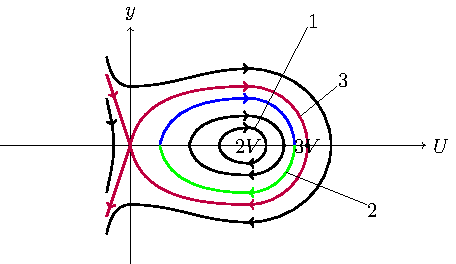
\includegraphics[width=0.5\linewidth]{fig/fig20.pdf}   
% \end{figure}
Математическим {образом солитона является гомоклиническая орбита} (траектория 3 на рисунке \ref{fig:phase_port}).

% 22.04

% Напомню, что дифференцирование в системе \eqref{eq:36} производится по бегущей координате. 

Вернемся к фазовому портрету. Неограниченные траектории лишены физического смысла, поэтому нас интересуют только ограниченные, то есть те, что находятся внутри петли сепаратрис, включая ее саму.

Возьмём траекторию вблизи состояния равновесия <<центр>> (на рисунке траектория 1). Она замкнутая, колебание близко к гармоническому. Колебание происходит на уровне $2V$. Таких колебаний континуум. 
\begin{figure}[H]
	\centering
	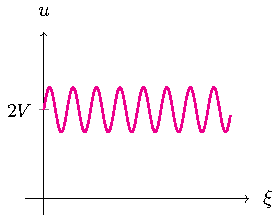
\includegraphics[scale=1.5]{img/soliton/2v}
\end{figure}

Выберем траекторию вблизи седла (на рисунке траектория 2), но все еще внутри гомоклинической орбиты. Выберем точку и положим при $\xi=0$ максимальную амплитуду. При движении по траектории к седлу (зеленым), u убывает. 
\begin{figure}[H]
	\centering
	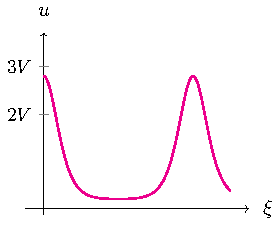
\includegraphics[scale=1.5]{img/soliton/25v}
\end{figure}

Около самого состояния равновесия скорость мала, движение в ее окрестности будет проходить медленно. В конце концов, при выходе из окрестности состояния равновесия, скорость опять увеличится. Мы получим профиль, так называемой, кноидальной волны, которая далека от гармонической. Волны такие из-за того, что система нелинейная. 

Если брать траектории все ближе к седлу, <<полка>> кноидального колебания будет увеличиваться. В конце концов, когда мы попадем на петлю:
\begin{figure}[H]
	\centering
	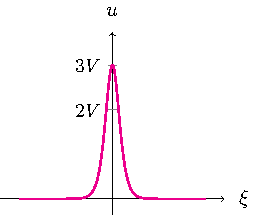
\includegraphics[scale=1.5]{img/soliton/3v}
\end{figure}
Для того, чтобы нарисовать профиль в области $\xi<0$, нужно пройти по траектории в обратном времени (время у нас $\xi$). Рисунок качественный, нарисован из понимания поведения функции на концах и знания максимальной амплитуды. 

Получившийся одиночный холм - это математический образ солитона.
% Точка 0 - решение, там нет пересечения траекторий, они стремятся туда асимптотически. 

\paragraph{Точный вид солитона.} Запишем уравнение \eqref{eq:s3:4} в виде одного:
\begin{equation}
	\beta\dv[2]{u}{\xi}=Vu-\frac{u^2}{2}
	\label{eq:s3:5}
\end{equation}
Решение будем искать в виде
\begin{equation}
	u=\frac{u_{max}}{\ch^2{(\xi / \Delta)}},
	\label{eq:s3:6}
\end{equation}
где введены параметры: $u_{max}, \Delta, V$ ($V$ скрыто в $\xi=x-Vt$). Подстановка \eqref{eq:s3:6} в \eqref{eq:s3:5} даёт
\begin{equation}
	\dv[2]{u}{\xi}=-2\frac{u_m}{\Delta^2}\frac{(3-2\ch^2{\xi / \Delta)}}{\ch^4{(\xi / \Delta)}}
	\label{eq:s3:7}
\end{equation}
\begin{gather*}
	\frac{2\beta u_m}{\Delta^2}\frac{(3-2\ch^2{(\xi / \Delta))}}{\ch^4{(\xi / \Delta)}}=\frac{u_m V}{\ch^2{(\xi / \Delta)}}-\frac{u_m^2}{2\ch^4{(\xi / \Delta)}}.
\end{gather*}
Приведя к общему знаменателю, получим
\begin{equation*}
	-2\beta[3-2\ch^2{(\xi / \Delta)}]=\Delta^2 \ch^2{(\xi / \Delta)}V-\frac{u_m \Delta^2}{2}
\end{equation*}
Чтобы это уравнение было тождеством, необходимо выполнение двух условий:
% Знаменатель не обращается в ноль.
\begin{equation}
	-6\beta=\frac{u_m \Delta^2}{2}
	\quad \Rightarrow \quad
	u_m \Delta^2= 12\beta,
	\label{eq:s3:8}
\end{equation}
\begin{equation}
	4\beta=\Delta^2V.
	\quad \Rightarrow \quad
	\Delta^2V=4\beta.
	\label{eq:s3:9}
\end{equation}
Параметры связаны, но их 3, а условия 2. Задав один, два других найдутся из \eqref{eq:s3:8} и \eqref{eq:s3:9}. 

$\beta$ характеризует дисперсию и не относится к самому солитону. $V$ -- скорость солитона, $u_m$ -- его высота, $\Delta$ оказывается шириной. Ширина солитона вычисляется на уровне $u=\frac{4u_m}{2+e}$. 
Из уравнения \eqref{eq:s3:9} следует, что, чем шире солитон, тем меньше его скорость, а из \eqref{eq:s3:8}, что чем шире солитон, тем меньше его амплитуда: $u_m=\frac{12\beta}{\Delta^2}$.

$V$ может принимать любые значения: это следствие непрерывности модели.

Если в диссипативной системе есть петля, то при изменении параметров она разрушается. Есть всего одна траектория, формирующая солитон. Солитоны столь интересны, потому что они устойчивы относительно большого числа начальных распределений. 

\subsubsection{Устойчивость солитона}
Замечание: рассмотрим уравнение Шредингера для определения статистического состояния. 
\begin{equation}
	\dv[2]{\psi}{x}+[u(x)+\epsilon]\psi=0.
	\label{eq::s310}
\end{equation}

$u(x)>0, ~u\rightarrow 0$ при $x\rightarrow \pm \infty$

Есть решение, когда спектр дискретный: $\epsilon=\epsilon_n, \psi, \psi' \rightarrow 0$ при $x\rightarrow \pm \infty$.\

Существует связь между \eqref{eq:41} и устойчивостью солитонов уравнения Кортевега - де Фриза. Надо подставить нормированное решение:
\begin{equation*}
	\dv[2]{\psi}{x}+[\frac{1}{6\beta}u(x,t)+\epsilon]\psi=0.
\end{equation*}

Покажем, что, если речь о солитоне, то $\epsilon$ не будет зависеть от t.
\begin{equation*}
	u(x,t)=-6\beta(\frac{\psi''}{\psi}+\epsilon),
\end{equation*}
здесь $'$ - дифференцирование по x. Подставим в уравнение Кортевега - де Фриза:
\begin{equation*}
	\pdv{u}{t}+u\pdv{u}{x}+\beta \pdv[3]{u}{x}=0.
\end{equation*}
\begin{equation}
	\psi^2\dv{\epsilon}{t}=(\psi'A-A\psi').
	\label{eq::s311}
\end{equation}
\begin{equation*}
	A(x,t)=6\beta(\frac1{\beta}\pdv{\psi}{t}-3\frac{\psi'\psi''}{\psi}+\psi'''-\frac{\epsilon}{6}\psi').
\end{equation*}

Проинтегрируем \eqref{eq:42} по переменной x в бесконечных пределах. Вспомним, что $\psi, \psi' \rightarrow 0$ при $x\rightarrow \pm \infty$. Получим:
\begin{equation*}
	\dv{\epsilon}{t}\int^{+\infty}_{-\infty}\psi^2dx=0.
\end{equation*}

В силу нормировки интеграл не равен нулю. Следовательно, $\dv{\epsilon}{t}=0$ и $\epsilon\neq \epsilon(t)$.
\begin{equation*}
	u(x,t)=u_{max}c\ch^{-2}(\frac{x-Vt}{\Delta}).
\end{equation*}

Здесь t можно выбрать любое. Положим, $t=0$.
\begin{equation}
	\psi''+(u_0 \ch^{-2}\alpha x+\epsilon)\psi=0.
	\label{eq::s312}
\end{equation}
\begin{equation*}
	u_0=\frac{u_m}{6\beta},~\alpha=\frac1{\Delta}.
\end{equation*}

Пользуясь случаем, передаем приветы и спасибо третьему тому Ландау-Лившица, параграф 23, задача 4, где это уравнение решено. Спектр:
\begin{gather*}
	\epsilon_n=-\alpha(s-n), n=0,1,2,\dots;~n<s \\ s=\frac12(-1+\sqrt{1+\frac{4u_0}{\alpha^2}})=\frac12(-1+\sqrt{\frac{4u_m\Delta^2}{6\beta}})=\frac12(-1+3)=1 \\ \epsilon_n=-\alpha(1-n) \\ n=0:~ \epsilon_0=-\alpha^2=-\frac{4u_m}{12\beta}.
\end{gather*}

Если в уравнение Шредингера подставить уравнение солитона, такому потенциалу соответствует одно собственное значение. Пусть в начальный момент есть распределение (положительно определенное, но не совпадающее с солитоном). Подставляя его в уравнения Шредингера, решив, получим столько $\epsilon_j$, сколько солитонов может существовать при таких начальных условиях.
\begin{figure}[H]
	\centering
	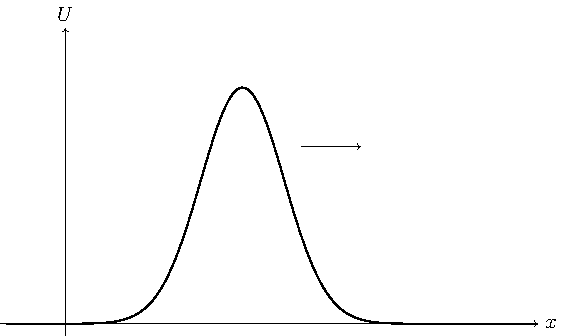
\includegraphics[width=0.4\linewidth]{fig/fig25.pdf}   
\end{figure}

Пусть $j=3$:
\begin{figure}[H]
	\centering
	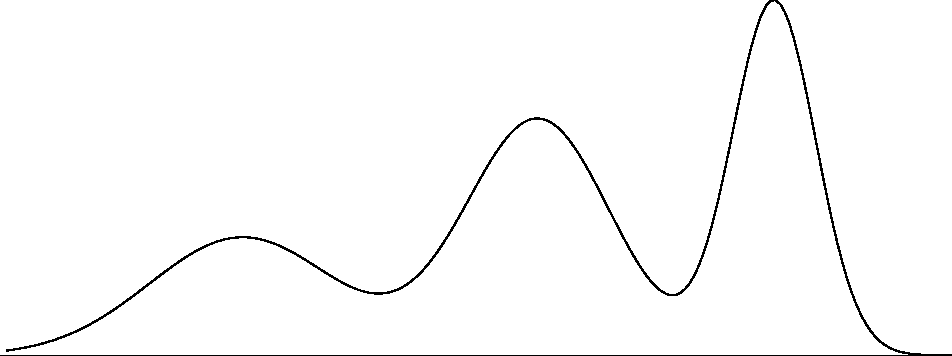
\includegraphics[width=0.4\linewidth]{fig/fig26.pdf}   
\end{figure}

Это обратная задача рассеяния. Качественные рассуждения: введем величину (из \eqref{eq:40}) $\sigma=\frac{\Delta^2 u_m}{12 \beta}=1$. Здесь $u_m$ характеризует нелинейность, а $\beta$ - дисперсию. Предположим, что при $t=0$ задали такое распределение, что $\sigma \ll 1$. Это означает малость $u_m$, мы находимся около стационарного состояния (около нуля). Если мы близки к линейной задаче, главную роль играют дисперсионные механизмы. Есть области прозрачности и непрозрачности. В области прозрачности фазовая скорость у каждой компоненты своя, пакет расплывается.  Приходим к единственному солитону.

Если  $\sigma \gg 1$, преобладает нелинейность. Она порождает новые гармоники. Переход к образованию состава из солитонов. Дисперсия ограничивает частоты, фронт стабилизируется.




% \section{Стационарные ударные волны}
% \label{sec:shock_waves}
% 	%!TEX root = ../lections.tex
Рассмотрим уравнение простой волны
\begin{equation}
	\pdv{u}{t}+u\pdv{u}{x}+\beta \pdv[3]{u}{x}-\underbrace{\nu\pdv[2]{u}{x}}_{\text{диссипация}}=0.
	\label{eq:shock:1}
\end{equation}

Здесь $\nu>0$ -- диссипация. Посмотрим, к чему приведет её учет. Если $\beta=0$, то уравнение называется уравнением Бюргерса. 

Будем искать решения в виде $\xi=x-Vt$ (их ещё называют стационарными решениями, так как профиль волны не меняется): 
\begin{equation*}
	-V\dv{u}{\xi}+u\dv{u}{\xi}+\beta\dv[3]{u}{\xi}-\nu\dv[2]{u}{\xi}=0.
\end{equation*}
Проинтегрируем:
\begin{equation*}
	\beta\dv[2]{u}{\xi}-\nu \dv{u}{\xi}+\frac{u^2}{2}-Vu=0.
\end{equation*}
Перепишем полученное уравнение в виде системы, дифференцирование по $\xi$ обозначая точкой:
\begin{equation}
	\begin{cases}
		\dot{u}=y \\
		\beta \dot{y} =\nu y-\frac{u^2}{2}+Vu.		
	\end{cases}
	\label{eq:shock:2}
\end{equation}

Система диссипативная. Найдем её состояния равновесия: $O_1(0,0)$, $O_2(2V,0)$. Несложный анализ (линеаризация) даст, что $O_1$ -- седло, а для $O_2$:
\begin{gather*}
	p^2-\frac{\nu}{\beta}p+\frac{V}{\beta}=0, \qquad p_{1,2}=\frac{\nu}{2\beta}\pm \sqrt{\frac{\nu^2}{4\beta^2}-\frac{V}{\beta}}.
\end{gather*}
Если $\frac{\nu^2}{4\beta^2}-\frac{V}{\beta}<0$, то имеем неустойчивый фокус.
\begin{equation*}
	\frac{\nu^2}{4\beta}=V \quad\rightarrow\quad \beta=\frac{\nu^2}{4V}.
\end{equation*}
Над этой кривой $\beta(\nu)$ состояние равновесия $O_2$ будет неустойчивым фокусом, а под -- неустойчивым узлом (см. рисунок ниже).
\begin{figure}[H]
	\centering
	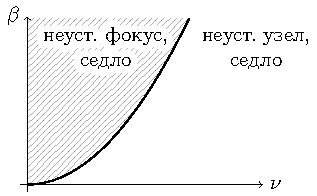
\includegraphics[scale=1.4]{img/shock_waves/beta_nu}
	\caption{Разбиение области параметров}
\end{figure}

Введем в рассмотрение функцию (полную энергию при $\nu=0$)
% Возьмем полную энергию при $\nu=0$:
\begin{equation*}
	V(u,y)=\beta\frac{y^2}{2}+\frac{u^3}{6}-V\frac{u^2}{2},
\end{equation*}
Линии уровня этой функции дают фазовый портрет при $\nu=0$.  Из существования этой функции следует, что система не имеет предельных циклов. 
Найдём производную $\dot{V}$ в силу системы \eqref{eq:shock:2}:
\begin{equation*}
	\dot{V}=\beta y \dot{y}+\frac{u^2}{2}\dot{u}-Vu\dot{u}=\nu y^2-\frac{u^2}{2}y+Vuy-Vuy+\frac{u^2}{2}y=\nu y^2\geqslant 0,
\end{equation*}
т.е. траектории системы пересекают линии уровня в сторону возрастания:
\begin{figure}[H]
	\centering
	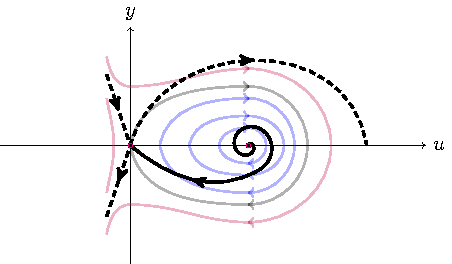
\includegraphics[scale=1.5]{img/shock_waves/phase_portrait}
\end{figure}
Как ведут себя устойчивые сепаратрисы седла? Ограниченное решение существует, оно единственно и соответствует траектории из фокуса в седло (см. рис. выше). 



% \begin{figure}[H]
% 	\centering
% 	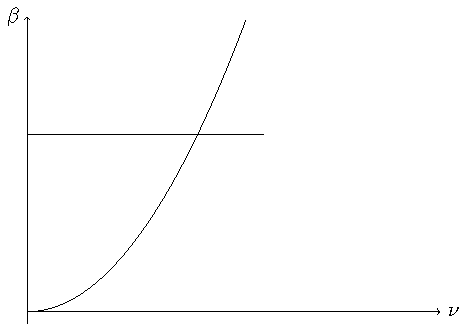
\includegraphics[width=0.4\linewidth]{fig/fig28.pdf}   
% \end{figure}

Зафиксируем $\beta$ и нарисуем профиль этой волны. Будем изучать траекторию, которая успеет сделать много витков, до того как придет в состояние равновесия. По прежнему $\nu\ll1$:
\begin{figure}[H]
	\centering
	% 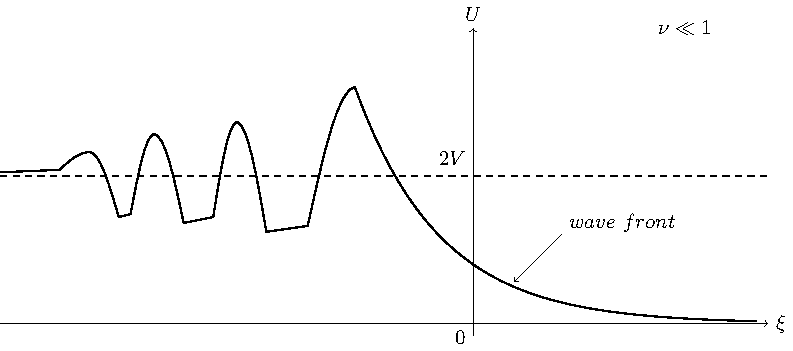
\includegraphics[width=0.6\linewidth]{fig/fig29.pdf} 
	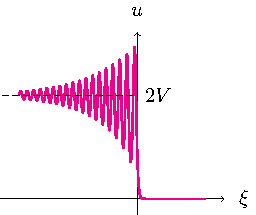
\includegraphics[scale=1.5]{img/shock_waves/shock} 
	\caption{Фронт волны <<переключает>> среду из $2V$ в $0$}
\end{figure}

Чем дальше от седла, тем ближе точки, выше и меньше полки. Это ударная волна.  Среда была в покое, прошел фронт и перебросил среду в новое состояние $2V$.

% Для красной траектории:
% \begin{figure}[H]
% 	\centering
% 	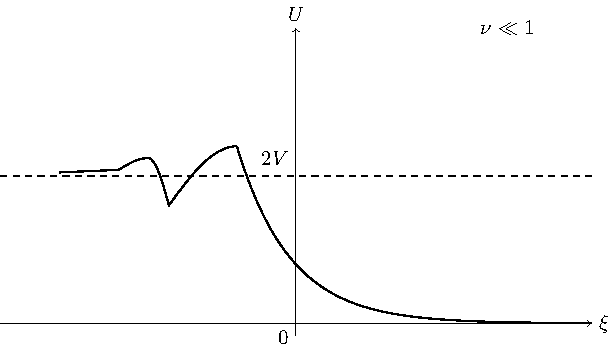
\includegraphics[width=0.6\linewidth]{fig/fig31.pdf}   
% \end{figure}

Если взять такой параметр $\beta$, что состояние равновесия $O_2$ будет узлом, то осцилляций не будет, но передний фронт останется. Волна, соответствующая единственной ограниченной траектории, идущей из неустойчивого состояния равновесия  --  узла в седло:
% \begin{figure}[H]
% 	\centering
% 	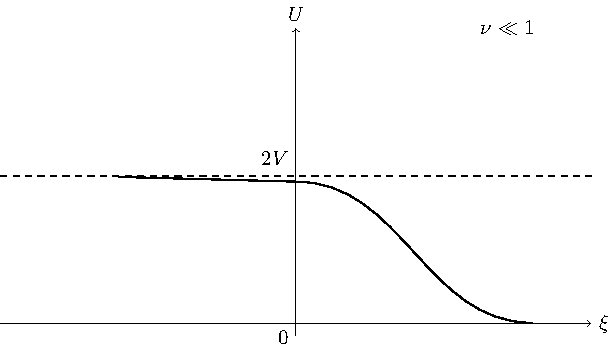
\includegraphics[width=0.6\linewidth]{fig/fig32.pdf}   
% \end{figure}
\begin{figure}[h]
\begin{minipage}[h]{0.49\linewidth}
\center{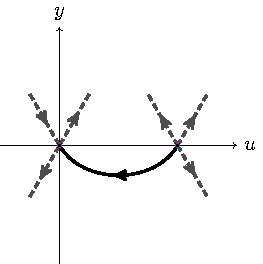
\includegraphics[scale=1.5]{img/shock_waves/phase_portrait_knot}}
\end{minipage}
\hfill
\begin{minipage}[h]{0.49\linewidth}
\center{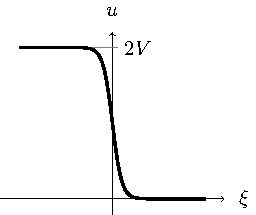
\includegraphics[scale=1.5]{img/shock_waves/shock_knot}}
\end{minipage}
	% \caption{Зависимость $\Re p$ от $k^2$ при $D_{1,2}\ne0$ и структура Тьюринга (справа)}
\end{figure}
% Здесь не будет осцилляций. Во всех случаях есть передний фронт.


% \newpage
% \section{Параметрические колебания}
% \label{sec:parametric_oscillations}
% % 29.04.19 
% 	%!TEX root = ../lections.tex
Ранее мы рассматривали системы, в которых под действием внешних силовых воздействий появлялись новые режимы. Они являлись неавтономными. Кроме них существует другой тип неавтономных систем и внешнего воздействия. Внешнее воздействие находится внутри системы и может изменять его параметры.
Такие системы -- параметрические, а их колебания - параметрические колебания. Пример системы -- маятник, длина которого периодически меняется, т.е. параметр длины меняется со временем. 

Параметрические системы делят на 2 важных класса: \textbf{резонансные} и \textbf{нерезонансные}. В резонансных системах период изменения параметров находится в целочисленном соотношении с периодом собственных колебаний. В таких системах в такт с изменением энергии, соответствующей собственным колебаниям, вносится энергия, вызванная работой внешнего воздействия. При определенных условиях это может приводить к эффекту раскачки колебаний за счет накапливающейся в системе энергии. Этот эффект лежит в основе работы параметрических усилителей и генераторов. 

К нерезонансным неколебательным параметрическим системам относятся системы, в которых параметры изменяются очень быстро или очень медленно по сравнению с характерным временными масштабами изменения переменных системы. Динамика линейных параметрических систем описывается системой линейных дифференциальных уравнений с периодическими коэффициентами. 

Далее будем рассматривать только линейные параметрические системы. В основе теории таких систем лежит так называемая \textbf{теория Флоке}. 

Рассмотрим двумерную систему
\begin{equation}
	\left\{\begin{aligned}
		&\dot{x_1}=p_{11}(t)\cdot x_1+p_{12}(t)\cdot x_2 \\
		&\dot{x_2}=p_{21}(t)\cdot x_1+p_{22}(t)\cdot x_2,	
	\end{aligned}\right.
	\label{eq:47}
\end{equation}
где $p_{jk}(t+T)=p_{jk}(t)$, то есть  коэффициенты периодически изменяются во времени. Запишем общее решение в матричном виде:
\begin{equation*}
	\vec{x} = X \vec{C}, 
\end{equation*}
где
\begin{gather*}
	\vec{x}= 
	\begin{pmatrix}
		x_1 \\
		x_2
	\end{pmatrix}
	,\quad
	\vec{C}= 
	\begin{pmatrix}
		c_1 \\
		c_2
	\end{pmatrix}
	,\quad
	X(t)= 
	\begin{pmatrix}
		\phi_1 ~~  \psi_1 \\
		\phi_2  ~~ \psi_2
	\end{pmatrix}.
\end{gather*}
Здесь векторы
\begin{gather*}
	\vec{\phi}= 
	\begin{pmatrix}
		\phi_1 \\
		\phi_2
	\end{pmatrix}
	,\quad
	\vec{\psi}= 
	\begin{pmatrix}
		\psi_1 \\
		\psi_2
	\end{pmatrix}
\end{gather*}
являются линейно независимыми, следовательно, образуют фундаментальную систему решений. 

Покажем, что в качестве $\phi,\psi$ можно выбрать такие функции, которые удовлетворяют начальным условиям:
\begin{gather}
	\phi_1(0)=1,\quad \psi_1(0)=0, \notag \\ 
	\phi_2(0)=0,\quad \psi_2(0)=1.		
	\label{eq:48}
\end{gather}

Согласно общей теории линейных дифференциальных уравнений вектора $\phi$, $\psi$  будут линейно независимы, если определитель Вронского не обращается в ноль:
\begin{gather*}
	W(t)= 
	\begin{vmatrix}
		\phi_1(t) ~~\psi_1(t) \\ 
		\phi_2(t) ~~\psi_2(t)
	\end{vmatrix}
	,
\end{gather*}
Для ограниченных $W$ верна формула Лиувилля-Остроградского:
\begin{equation}
	W(t)=W(0)\exp\qty[\int_0^t(p_{11}(t)+p_{22}(t))\dd{t}].
	\label{eq:49}	
\end{equation}

Для начальных условий \eqref{eq:48} получается $W(0)=1$, отсюда следует, что вронскиан отличен от нуля, значит $\phi$, $\psi$ линейно независимы и образуют ФСР.

Поскольку $p_{jk}(t)$ являются периодическими, то вектора $\vec{\phi}(t+T)$, $\vec{\psi}(t+T)$ также линейно не зависимы и являются решением системы \eqref{eq:47}. Как всякое решение, эти вектора можно выразить через ФСР:
\begin{gather}
	\left\{\begin{aligned}
	\vec{\phi}(t+T)=a\vec{\phi}(t)+b\vec{\psi}(t), \\ 
	\vec{\psi}(t+T)=c\vec{\phi}(t)+d\vec{\psi}(t),			
	\end{aligned}\right.
	\label{eq:50}
\end{gather}
где $a,b,c,d$ -- некоторые константы. Их можно найти, подставив $t=0$ и учтя начальные условия \eqref{eq:48}:
\begin{equation}
	a=\phi_1(T),~ b=\phi_2(T),~ c=\psi_1(T),~ d=\psi_2(T).
	\label{eq:51}	
\end{equation}

Соотношения \eqref{eq:51} говорят о том, что константы могут быть найдены, если известно общее решение $\vec\phi, \vec\psi$.

Покажем, что существуют такие константы $a,b,c,d$, что для системы  \eqref{eq:47} справедливо:
\begin{equation}
	\vec{x}(t+T)=s\vec{x}(t),
	\label{eq:52}	
\end{equation}
т.е. через период решение повторяется с точностью до множителя.

Поскольку любое решение системы \eqref{eq:47} можно получить из общего решения надлежащим выбором констант, то
\begin{equation}
	\vec{x}(t)=A\vec{\phi}(t)+B\vec{\psi}(t),
	\label{eq:53}	
\end{equation}
% 
% Запишем состояние этого вектора в момент времени $t+T$:
\begin{equation}
	\vec{x}(t+T)=A\vec{\phi}(t+T)+B\vec{\psi}(t+T)
	\label{eq:54}	
\end{equation}
С другой стороны, подставим \eqref{eq:53} и \eqref{eq:54} в \eqref{eq:52}:
\begin{equation}
	A\vec{\phi}(t+T)+B\vec{\psi}(t+T)=s\qty[A\vec{\phi}(t)+B\vec{\psi}(t)].
	\label{eq:55}	
\end{equation}
Теперь используем \eqref{eq:50}:
\begin{equation}
	\qty[A(a-s)+Bc]\vec{\phi}(t)+\qty[Ab+B(d-s)]\vec{\psi}(t) \equiv 0.
	\label{eq:56}	
\end{equation}
Для выполнения равенства при любом $t$ нужно, чтобы скобки с коэффициентами обратились в ноль:
\begin{equation}
	\left\{\begin{aligned}
		&A(a-s)+Bc=0 \\
		&Ab+B(d-s)=0.		
	\end{aligned}\right.
	\label{eq:57}
\end{equation}
Это СЛАУ относительно коэффициентов $A$, $B$. Раскрываем определитель:
\begin{equation}
	s^2-(a+d)s+ad-bc=0.
	\label{eq:58}	
\end{equation}
Оказывается, что $ad-bc$ всегда можно найти, не находя общего решения.

Вернемся к вронскиану. Подсчитаем его в момент времени $T$:
\begin{gather*}
	W(T)= 
	\begin{vmatrix}
		\phi_1(T) & \psi_1(T) \\ 
		\phi_2(T) & \psi_2(T)
	\end{vmatrix}
	=
	\begin{vmatrix}
		a & c \\ 
		b & d
	\end{vmatrix}
	=ad-bc.
\end{gather*}
с другой стороны,
\begin{eqnarray*}
	W(T)=\underbrace{W(0)}_{\text{=1}}\exp\qty[\int_0^T(p_{11}(t)+p_{22}(t))\dd{t}] \\
\end{eqnarray*}
\begin{equation}
	ad-bc=\exp\qty[\int_0^T\qty(p_{11}(t)+p_{22}(t))\dd{t}].
	\label{eq:59}
\end{equation}
Так как $p_{11}, p_{22}$ мы знаем из постановки конкретной задачи, то $ad-bc$ всегда найдём.

Предположим, что \eqref{eq:58} не имеет кратных корней, следовательно, существует два значения мультипликатора и два
решения:
\begin{gather}
	\vec{x}_1(t+T)=s_1\vec{x}_1(t) \notag \\ 
	\vec{x}_2(t+T)=s_2\vec{x}_2(t).		
	\label{eq:60}
\end{gather}
Таким образом, решение воспроизводит себя через период с точностью до множителя.
\begin{gather}
	\vec{x}_1(t+nT)=(s_1)^n\vec{x}_1(t) \notag \\ 
	\vec{x}_2(t+nT)=(s_2)^n\vec{x}_2(t).		
	\label{eq:61}
\end{gather}

Покажем, что решения $\vec{x}_1,\vec{x}_2$ можно представить в следующем виде:
\begin{gather}
	\vec{x}_1(t)=e^{\lambda_1t}\vec{\Phi}_1(t), \qquad
	\vec{x}_2(t)=e^{\lambda_2t}\vec{\Phi}_2(t),		
	\label{eq:62}
\end{gather}
где $\lambda$ -- некоторые числа, которые называются характеристическими, а вектора $\vec{\Phi}$ имеют вид 
\begin{gather*}
	\vec{\Phi}_1(t)= 
	\begin{pmatrix}
		\Phi_{11} \\
		\Phi_{21}
	\end{pmatrix}
	,\quad
	\vec{\Phi}_2(t)= 
	\begin{pmatrix}
		\Phi_{12} \\
		\Phi_{22}
	\end{pmatrix}
	,
\end{gather*}
и являются периодическими с периодом $T$:
\begin{equation}
	\Phi_{kj}(t+T)=\Phi_{kj}(t),
	\label{eq:63}
\end{equation}
а характеристические числа представляются в следующем виде:
\begin{gather}
	\lambda_j=\frac{1}{T}\,\mathrm{Ln}\,s_j=\frac1{T}\qty[\vphantom{\bigg|}\ln|s_j|\pm i\qty(\vphantom{\big|}\arg s_j +2\pi k)], \quad
	\begin{aligned}
		&j=1,2, \\
		&k=0,\pm 1, \pm 2, \ldots	
	\end{aligned}
	\label{eq:64}
\end{gather}
$s$ -- мультипликаторы, которые могут быть комплексными, поэтому присутствует аргумент комплексного числа.

Покажем справедливость \eqref{eq:63}. Из \eqref{eq:62}:
\begin{equation*}
	\vec{\Phi}_j(t)=e^{-\lambda_j t}\vec{x}_j(t),
\end{equation*}
но $\vec{x}_j$ можно выразить из \eqref{eq:60}:
\begin{gather*}
	\vec{x}_j(t+T)=s_j\vec{x}_j(t)=e^{\lambda_j T}\vec{x}_j(t), \\
	\vec{\Phi}_j(t+T)=e^{-\lambda_j(t+T)}\vec{x}_j(t+T)=e^{\lambda_j T}\vec{x}_j(t)e^{-\lambda_j(t+T)}=\vec{x}_j(t)e^{-\lambda_j t}=\vec{\Phi}_j(t).
\end{gather*}

С другой стороны, $\vec{x}_j$ образуют ФСР, поэтому общее решение можно записать в виде
\begin{equation}
	\vec{x}(t)=\sum_{j=1}^2 c_j e^{\lambda_j t}\vec{\Phi}_j(t).
	\label{eq:65}
\end{equation}

Это основное соотношение ЛДУ с переменными параметрами. Здесь $\Phi$ -- функции Флоке. 

\paragraph{Замечание. } Теория Флоке может быть применена к предельным циклам, так как  они являются переодическим решением. 




\subsection{Отображение через период}

С точки зрения теории динамических систем, \eqref{eq:47} представляет собой неавтономную систему, следовательно, порождает точечное отображение 
% \begin{figure}[H]
% 	\centering
% 	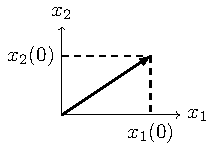
\includegraphics[scale=1.5]{img/parametric_oscillations/x_to_v}
% \end{figure}

\begin{wrapfigure}{l}{6cm}
	\centering
    \vspace{-1ex}%сместить картинку немного вверх  относительно текста
    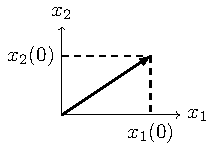
\includegraphics[scale=1.5]{img/parametric_oscillations/x_to_v}
    % \caption{Предельная нагрузка настила по условию прогиба}
    \label{img02}
\end{wrapfigure}
$$g^t:\mathds{R}^2\rightarrow \mathds{R}^2.$$
Под действием системы \eqref{eq:47} вектор $\vec{x}(0)$ переходит в другой вектор $\vec{v}(t)$:
\begin{equation*}
	g^t\,\vec{x}(0)=\vec{v}(t).
\end{equation*}
Если $t=0: \,\vec{x}(0)=\vec{v}(0)$.
В силу теории Флоке наибольший интерес представляет отображение через период, т.е. $g^T$. Заметим, что решение $x_1=0, x_2=0$ является неподвижной точкой этого отображения. Более того, с точки зрения неавтономной системы, это периодическое решение любого периода. 

Воспользуемся соотношением Флоке (см. \eqref{eq:65}):
\begin{gather}
	x_1(t)=C_1 e^{\lambda_1 t}\Phi_{11}(t)+C_2 e^{\lambda_2 t}\Phi_{12}(t) \notag \\ 
	x_2(t)=C_1 e^{\lambda_1 t}\Phi_{21}(t)+C_2 e^{\lambda_2 t}\Phi_{22}(t).	
	\label{eq:66}
\end{gather}
Пусть $x_1(0)=x_1$, $x_2(0)=x_2$. Подставим $t=0$ в \eqref{eq:66}, находим $C_1^0, C_2^0$ через получившуюся СЛАУ. 
% Задаем точку, находим ее образ через период:
% \begin{gather}
% 	x_1(t)=C_1^0 e^{\lambda_1 t}\Phi_{11}(t)+C_2^0 e^{\lambda_2 t}\Phi_{12}(t) \notag \\ 
% 	x_2(t)=C_1^0 e^{\lambda_1 t}\Phi_{21}(t)+C_2^0 e^{\lambda_2 t}\Phi_{22}(t),		
% 	\label{eq:67}
% \end{gather}

Используя \eqref{eq:53}, \eqref{eq:62} и начальные условия \eqref{eq:48}, а также связь  $A,B$ с $a, b, c, d$, получим: 
\begin{gather}
	\Phi_{11}(0)=A_1,~\Phi_{21}(0)=B_1,~\Phi_{12}(0)=A_2,~\Phi_{22}(0)=B_2.	
\end{gather}
\begin{equation}
	g^T\rightarrow
	\left\{\begin{aligned}
		x_1(T)=a x_1(0)+c x_2(0) \\
		x_2(T)=b x_1(0)+d x_2(0)		
	\end{aligned}\right. \quad\Rightarrow\quad
	\vec{x}(T)=G \vec{X}(0),
	\label{eq:68}
\end{equation}
где
\begin{gather*}
	G=
	\begin{pmatrix}
		a ~c \\
		b ~d \\
	\end{pmatrix}
	,\quad
	a=\phi_1(T), ~ b=\phi_2(T), ~
	c=\psi_1(T), ~ d=\psi_2(T).
\end{gather*}

Траектории системы порождают точечное линейное отображение, где роль дискрета играет период $T$. Далее
займемся исследованием устойчивости неподвижных точек. 


\subsection{Устойчивость нулевого решения}
Рассмотрим точечное отображение \eqref{eq:68}. Поведение $g^T$ зависит от мультипликаторов $s_{1,2}$. Пусть $s_1, s_2$ -- действительные: тогда \eqref{eq:68} с помощью преобразования можно привести к диагональному виду:
\begin{equation}
	\left\{\begin{aligned}
		u_1(T)=s_1 u_1(0) \\
		u_2(T)=s_2 u_2(0)		
	\end{aligned}\right.
	\label{eq:unn}
\end{equation}
\begin{enumerate} 
	\item Поскольку мультипликаторы $s_1, s_2$ соответствуют решениям неавтономной  системы \eqref{eq:47}, они удовлетворяют условию $s_1\cdot s_2>0$;
	\item Если $|s_j|<1$, неподвижная точка устойчива, если $|s_j|>1$ - неустойчива. Если $|s_i|<1, |s_j|>1,~ i\ne j$, то точка -- седло. 
\end{enumerate} 

\begin{figure}[H]
	\centering
	\begin{minipage}{0.65\linewidth}
		\textbf{Устойчивость без перескоков. }

		Пусть $0<s_j<1$. Тогда под действием отображения вектор уменьшит длину и повернется.
		При любом начальном условии каждое следующее действие отображения приближает решение к нулю, следовательно, решение устойчивое.
	\end{minipage}
	\begin{minipage}{0.34\linewidth}
		\centering
		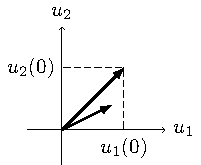
\includegraphics[scale=1.5]{img/parametric_oscillations/sj_1}	
	\end{minipage}		
\end{figure}

\begin{figure}[H]
	\centering
	\begin{minipage}{0.65\linewidth}
		\textbf{Устойчивость с перескоками. }

		Теперь $-1<s_j<0$. При первом отображении вектор уменьшит длину и переместится в отрицательную область, при втором уменьшит длину и
		переместится в положительную, и так далее: будут скачки. Решение устойчивое.
	\end{minipage}
	\begin{minipage}{0.34\linewidth}
		\centering
		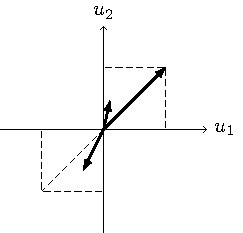
\includegraphics[scale=1.5]{img/parametric_oscillations/sj_2}
	\end{minipage}		
\end{figure}

\begin{figure}[H]
	\centering
	\begin{minipage}{0.65\linewidth}
		\textbf{Неустойчивость без перескоков. }

		$0<|s_1|<1$, $|s_2|>1$. По одной координате растяжение, а по другой сжатие. Вектор асимптотически прижимается к
		оси ординат.
	\end{minipage}
	\begin{minipage}{0.34\linewidth}
		\centering
		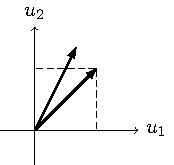
\includegraphics[scale=1.5]{img/parametric_oscillations/sj_3}   
	\end{minipage}		
\end{figure}

\begin{figure}[H]
	\centering
	\begin{minipage}{0.65\linewidth}
		\textbf{Неустойчивость c перескоками. } 

		$-1<|s_1|<0$, $|s_2|<-1$. Вектор прижимается к оси ординат и растягивается c перескоками.
	\end{minipage}
	\begin{minipage}{0.34\linewidth}
		\centering
		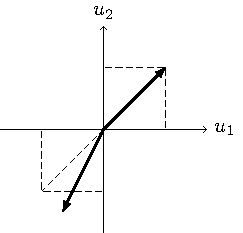
\includegraphics[scale=1.5]{img/parametric_oscillations/sj_4}   
	\end{minipage}		
\end{figure}

% 29.04
% Линейным преобразованием систему можно привести к нормальной форме.
% \begin{equation}
% 	u_j(T)=s_j u_j(0), ~j=1,2.
% 	\label{eq:69}
% \end{equation}

% $|s|<1$ - длина вектора меняется.
\paragraph{Комплексно-сопряженные корни. } Теперь $s_j=\alpha \pm i\beta$. Поскольку мультипликаторы являются комплексно сопряженными, переменные $u_j(T), u_j(0)$ будут комплексными функциями:
\begin{gather}
	u_j(0)=u(0)\pm iv(0) \notag \\ 
	u_j(T)=u(T)\pm iv(T).		
	\label{eq:71}
\end{gather}

Подставляя $s_j=\alpha \pm i\beta$ и уравнения \eqref{eq:71} в \eqref{eq:unn}, разделяя реальную и мнимую части, получим:
\begin{gather}
	u(T)=\alpha u(0)- \beta v(0) \notag \\ 
	v(T)=\beta u(0)+ \alpha v(0).		
	\label{eq:72}
\end{gather}
Приведём уравнения к нормальной форме. Для этого перейдем к полярным координатам:
\begin{gather}
	\begin{aligned}
		&u=\rho \cos{\phi}\\
		&v=\rho \sin{\phi}\\
		&s=\alpha \pm i\beta=|s|e^{\pm i \omega}
	\end{aligned}\qquad\Rightarrow\qquad
	\begin{aligned}
	 	&|s|=\sqrt{\alpha^2+\beta^2}\\
	 	&\alpha=|s|\cos{\omega}\\
	 	&\beta=|s|\sin{\omega}
	 \end{aligned} 		
	 \label{eq:73}
\end{gather}
Перепишем уравнения \eqref{eq:72} в полярных координатах:
\begin{equation}
	\left\{\begin{aligned}
		&\rho(T)\cos{\phi(T)}=\alpha \rho(0)\cos{\phi(0)}-\beta \rho(0)\sin{\phi(0)} \\
		&\rho(T)\sin{\phi(T)}=\beta \rho(0)\cos{\phi(0)}+\alpha \rho(0)\sin{\phi(0)}.
	\end{aligned}\right.
	\label{eq:74}
\end{equation}
Из этой системы находятся $\rho(T)$ и $\phi(T)$:
\begin{equation}
	\left\{\begin{aligned}
		&\phi(T)=\phi(0)+\omega \\
		&\rho(T)=|s|\rho(0).
	\end{aligned}\right.
	\label{eq:75}
\end{equation}

Эта система задает отображение $g^T$. Полярный угол $\phi$ меняется за период на $\omega$, а начальная величина вектора $\rho(0)$ изменяется в зависимости от s. 

\begin{figure}[H]
	\centering 
	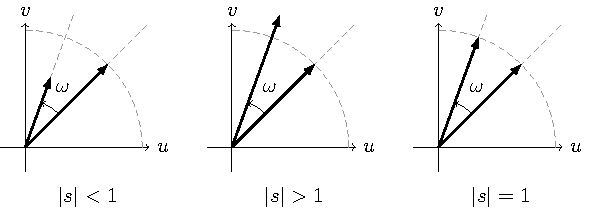
\includegraphics[scale=1.5]{img/parametric_oscillations/sj_vu} 
\end{figure}

Если $|s|<1$, вектор поворачивается на угол $\omega$ и сокращается в длину. Состояние равновесия и соответствующая ему неподвижная точка $x_1=x_2=0$ являются асимптотически устойчивыми.

$|s|>1$, состояние равновесия неустойчивое, вектор поворачивается и растягивается.

$|s|=1$, вектор поворачивается, длина его не меняется: вектор, пройдя период, может либо совпасть с начальным, либо нет. В зависимости от этого решение будет периодическим или квазипериодическим.

Таким образом, состояние равновесия или периодическая траектория любого периода в параметрической системе может быть устойчивой либо не устойчивой.

\subsection{Основные режимы линейной параметрической системы}

Поскольку система линейная, из условия устойчивости состояния равновесия вытекают все остальные свойства линейных параметрических систем, а именно:
\begin{enumerate} 
	\item Параметрическая система, находящаяся в начальный момент в состоянии равновесия, останется в этом состоянии при $\forall t>0$, поскольку состояние равновесия $x_1=x_2=0$ существует всегда в линейной системе. Параметрическую систему, находящуюся в состоянии равновесия, нельзя вывести из этого состояния, изменяя ее параметры. Пример -- маятник на нитке: дергая за нитку, маятник нельзя раскачать;
	\item Состояние равновесия параметрической системы может быть как устойчивым, так и не устойчивым;
	\item Если параметры системы таковы, что она неустойчива и система выведена из состояния равновесия, то в ней возникают колебания, амплитуда которых экспоненциально возрастает.  Процесс возрастания размахов колебаний при периодическом нарастании колебаний называется параметрическим резонансом.
\end{enumerate} 

\subsection{Параметрические колебания. Резонанс.}
Установим условие существования параметрического резонанса в одном частном, но важном случае. Рассмотрим систему \eqref{eq:47} в случае, когда $p_{11}(t) \equiv0$, $p_{12}(t)\equiv 1$, $p_{22}(t) \equiv 0$, тогда система примет вид:
\begin{equation}
	\left\{\begin{aligned}
		&\dot{x_1}=x_2 \\
		&\dot{x_2}=p_{21}(t)x_1.
	\end{aligned}\right.
	\label{eq:76}
\end{equation}
Система \eqref{eq:76} охватывает уравнения Матьё и Хилла. 

Поведение системы определяют мультипликаторы, а они, в свою очередь, определяются характеристическим уравнением:
\begin{gather*}
	s^2-(a+d)s+(ad-bc)=0, \\
	ad-bc=\exp\qty[\int_0^T(p_{11}(t)+p_{22}(t))\dd{t}]=1.		
\end{gather*}

Фактически, варьируются только коэффициенты $a$ и $d$. Введем контрольный параметр $2P=a+d$, тогда
\begin{gather*}
	s^2-2Ps+1=0.		
\end{gather*}

Проанализируем поведение $s$.
Пусть $|P|<1$:
\begin{gather*}
	s_{1,2}=P\pm i\sqrt{1-P^2}, \\
	|s|=1.		
\end{gather*}
Неподвижная точка отображения $g^T$ будет эллиптической. 
Достаточно рассмотреть только $x_1(t)$:
\begin{equation}
	x_1(t)=c_1e^{\lambda_1 t}\Phi_{11}(t)+c_2e^{\lambda_2 t}\Phi_{12}(t).
	\label{eq:77}
\end{equation}

Поскольку $|s|=1$, характеристические показатели $\lambda$ связаны с $s$, из  \eqref{eq:64} следует, что
\begin{equation*}
	\lambda_1=\frac{q}{T}i, \quad \lambda_2=-\frac{q}{T}i, \qq{где}
	q=|\arg s_j+2\pi k|
\end{equation*}
$\lambda$ чисто мнимые, $x$ действительные, следовательно, $c_1$, $c_2$, $\Phi_{11}$, $\Phi_{12}$ должны быть комплексными:
\begin{equation}
	\begin{aligned}
		&c_1=\frac{A}{2}e^{ic} \\
		&c_2=\frac{A}{2}e^{-ic}
	\end{aligned} \qquad\qquad
	\begin{aligned}
		&\Phi_{11}=h(t)e^{i\varkappa(t)}\vphantom{\frac{A}{2}} \\
		&\Phi_{12}=h(t)e^{-i\varkappa(t)}\vphantom{\frac{A}{2}}
	\end{aligned}
	\label{eq:78}
\end{equation}
Здесь $h(t)$, $\varkappa(t)$ -- периодические с периодом изменения параметров $T$, что следует из теории Флоке. Подставляя \eqref{eq:78} в \eqref{eq:77}, получим:
\begin{equation}
	x_1(t)=A\,h(t)\,\cos (\frac{q}{T}t+c+\varkappa(t)).
	\label{eq:79}
\end{equation}
Вспомним косинус суммы, чтобы выделить соответственные временные масштабы:
\begin{equation}
	x_1(t)=H(t)\cos(\frac{q}{T}t+c)+F(t)\sin(\frac{q}{T}t+c),
	\label{eq:80}
\end{equation}
где
\begin{gather*}
	H(t)=Ah(t)\cos \varkappa(t), \qquad
	F(t)=-Ah(t)\sin \varkappa(t).		
\end{gather*}

В \eqref{eq:80} функции  $H(t)$ и $F(t)$ периодичны с периодом $T$. Есть два временных масштаба: $T_1=T$ и $T_2=\frac{2\pi}{q}T$, которым отвечают частоты $\omega_1$ и $\omega_2$ соответственно.

Заметим, что $\frac{\omega_1}{\omega_2}=\frac{2\pi}{q}$, откуда вытекает, что, если $\frac{2\pi}{q}$ -- рациональное число, то $x_1(t)$ -- периодическая функция, если иррациональное, то $x_1(t)$ -- квазипериодическая функция. 

Таким образом, при выполнении $P<1$, в системе \eqref{eq:76} реализуются ограниченные колебания, которые называются параметрическими.

Пусть $|P|>1$.

Из характеристического уравнения $s_1 \cdot s_2=1$, они действительны. Для определенности $|s_1|>1,~ |s_2|<1$.

Теперь рассмотрим случай $P>1$. Действует отображение $g^T$:
\begin{figure}[H]
	\centering
	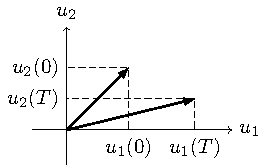
\includegraphics[scale=1.5]{img/parametric_oscillations/Pbigger}  
\end{figure}

По переменной $u_1$ увеличение вектора, по $u_2$ - уменьшение. Процесс повторяется. Вектор вытягивается и прижимается к оси абсцисс. Если $n\rightarrow \infty$ (число итераций): $u_2(nT)\rightarrow 0,~u_1(nT)\rightarrow \infty$. В системе реализуется параметрический резонанс. 

Получим приближенное соотношение для $x_1(t)$:
\begin{gather*}
	\lambda_1=\frac{1}{T}\ln s_1 >0, \\
	\lambda_2=\frac{1}{T}\ln s_2=\frac{1}{T}\ln(\frac{1}{s_1})=-\frac{1}{T}\ln s_1 <0.
\end{gather*}

Функция Флоке ограничена, отсюда следует, что
\begin{equation*}
	x_1(t)\approx c_1\cdot\exp(\frac{1}{T}\ln s_1 \, t)\cdot\Phi_{11}(t).
\end{equation*}
\begin{figure}[H]
	\centering
	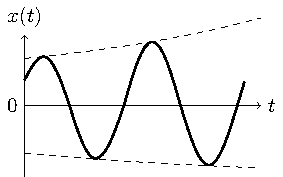
\includegraphics[scale=1.5]{img/parametric_oscillations/x_t}  
\end{figure}

В начальный момент система должна быть выведена из равновесия. Это геометрическая прогрессия, экстремумы функции лежат на экспоненте. 
\begin{itemize}
	\item В линейном осцилляторе экстремумы на прямых;
	\item Если линейный осциллятор в покое, мы можем его раскачать;
\end{itemize}

Пусть $s_1,s_2<0,~|s_1|>1,~|s_2|<1$:
\begin{figure}[H]
	\centering
	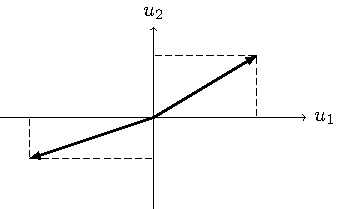
\includegraphics[scale=1.5]{img/parametric_oscillations/skok} 
\end{figure}

Вектор вернется через 2 итерации, период 2T, экстремумы отстоят на период.
\begin{figure}[H]
	\centering
	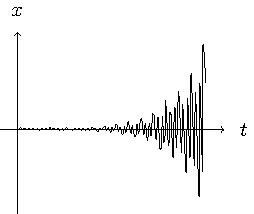
\includegraphics[scale=1.5]{img/parametric_oscillations/res}
\end{figure}

Пусть $|P|=1$. В этом случае, если $P=1$, то $s_1=s_2=1$; если $P=-1$, то $s_1=s_2=-1$. Корни кратные, мы такое не рассматривали. Решение в этом случае задается в виде:
\begin{gather*}
	x_1(t)=c_1 e^{\lambda t}\Phi(t)+c_2te^{\lambda t}\Phi(t), \qq{где}
	\lambda=\frac{1}{T}\ln|s|.
\end{gather*}

На границе неустойчивость и состояние равновесия $x_1=x_2=0$ является неустойчивым.

\subsection{Параметрические колебания маятника}
Рассмотрим маятник, у которого длина периодически меняется $l(t+T)=l(t)$, $\delta$ характеризует диссипацию:
\begin{equation}
	\ddot{\varphi}+2\delta \dot{\varphi}+\frac{g}{l(t)}\varphi=0.
	\label{eq:81}
\end{equation}
Зададим вид функции $l(t)$ кусочно-линейной аппроксимацией,  считая, что длина меняется мгновенно:
\begin{equation*}
	l(t)=
	\left\{\begin{aligned}
		&l_0-\frac{a}{2}, \qquad 0 \leq t \leq \frac{T}{2} \\
		&l_0+\frac{a}{2}, \qquad \frac{T}{2} \leq t \leq T		
	\end{aligned}\right.
\end{equation*}
Мы задали только на $t=0\dots T$, далее периодично. Такое колебание называется меандром. Введём обозначения
\begin{equation}
	% l_0=\frac{a}{2}>0,~
	\omega_1^2=\frac{g}{l_0-\frac{a}{2}}, \qquad \omega_2^2=\frac{g}{l_0+\frac{a}{2}} \quad \Rightarrow \quad
	\omega^2(t)=
	\left\{\begin{aligned}
		\omega^2_1, 0 \leq t \leq \frac{T}{2} \\
		\omega^2_2, \frac{T}{2} \leq t \leq T		
	\end{aligned}\right.
	\label{eq:83}	
\end{equation}

Рассмотрим консервативный случай ($\delta=0$). Перепишем \eqref{eq:81} в виде:
\begin{equation}
	\left\{\begin{aligned}
		&\dot{\varphi}=y \\
		&\dot{y} =-\omega^2(t)\varphi.	
	\end{aligned}\right.
	\label{eq:82}
\end{equation}
Система \eqref{eq:82} является частным случаем рассмотренного ранее случая, когда, $p_{21}=\omega^2(t)$. Для построения областей надо построить границы $P=\pm 1$, найдя $a$, $d$. Они являются элементами матрицы $G$, которая задает $g^T$. Поскольку система является кусочно-линейной, можно представить матрицу в виде $G=G_1\cdot G_2$, где $G_1$ действует на интервале от 0 до $\frac{T}{2}$, $G_2$ от $\frac{T}{2}$ до $T$. 

\paragraph{Матрица $G_1$. } Здесь $\omega^2(t)\equiv\omega_1^2$, решая \eqref{eq:82}, получим:
\begin{gather*}
	\varphi_1(t)\equiv A_1 \cos(\omega_1 t) + B_1\sin(\omega_1 t), \\
	\varphi_2(t)\equiv -A_1 \omega_1\sin(\omega_1 t) + \omega_1 B_1\cos(\omega_1 t).
\end{gather*}
Положим $\varphi_1(0)=1$, $\varphi_2(0)=0$, $A_1=1,~B_1=0$. Искомое решение примет вид: 
\begin{equation}
	\left\{\begin{aligned}
		&\varphi_1(t) = \cos(\omega_1 t) \\
		&\varphi_2(t) = - \omega_1\sin(\omega_1 t).		
	\end{aligned}\right.
	\label{eq:84}	
\end{equation}
Аналогично находится второе решение c начальным условием $\psi_1(0)=0$, $\psi_2(0)=1$:
\begin{gather}
	\left\{\begin{aligned}
		\psi_1(t) = \frac{\sin(\omega_1 t)}{\omega_1} \\
		\psi_2(t) = \cos(\omega_1 t).		
	\end{aligned}\right.
	\label{eq:85}	
\end{gather}
Подставляя $t=\frac{T}{2}$, найдем элементы $G_1$:
\begin{equation}
	\begin{aligned}
		&a_1 = \cos(\omega_1 \frac{T}{2})\quad
		&b_1 = \frac{\sin(\omega_1 \frac{T}{2})}{\omega_1}\\
		&c_1 = -\omega_1 \sin(\omega_1 \frac{T}{2}) \quad
		&d_1 = \cos(\omega_1 \frac{T}{2}),	
	\end{aligned}
	\label{eq:86}	
\end{equation}
Или в более кратком виде
\begin{gather*}
	G_1= 
	\begin{pmatrix}
		\cos \alpha~~~~~\frac{\sin\alpha}{\omega_1} \\
		-\omega_1 \sin \alpha~~\cos \alpha
	\end{pmatrix}
	, \qq{где}
	\alpha=\omega_1 \frac{T}{2}.	
\end{gather*}

\paragraph{Матрица $G_2$. } Вид устанавливается аналогично:
\begin{gather*}
	G_2= 
	\begin{pmatrix}
		\cos \beta~~~~~\frac{\sin\beta}{\omega_2} \\
		-\omega_2 \sin \beta~~\cos \beta
	\end{pmatrix}
	, \qq{где}
	\beta=\omega_2 \frac{T}{2}.	
\end{gather*}

\paragraph{Матрица $G=G_1\cdot G_2$. } Получили матрицу, элементы которой имеют вид:
\begin{gather*}
	a=\cos \alpha \cdot \cos \beta -\frac{\omega_1}{\omega_2} \sin \alpha \cdot \sin \beta, \\
	b=-\omega_2 \cos \alpha \cdot \sin \beta - \omega_1 \sin \alpha \cdot \sin \beta, \\
	c=\frac{\sin \alpha \cdot \cos \beta}{\omega_1}+\frac{\cos \alpha \cdot \sin \beta}{\omega_2}, \\
	d=\cos \alpha \cdot \cos \beta-\frac{\omega_2}{\omega_1}\sin \alpha \cdot \sin \beta,
\end{gather*}
Тогда можем найти параметр $P$:
\begin{equation}
	2P=a+d=2\cos \alpha\cdot \cos \beta - \frac{\omega_1^2+\omega_2^2}{\omega_2 \omega_1} \sin \alpha \cdot \sin \beta.
	\label{eq:87}	
\end{equation}

Введем более физичные параметры: собственная частота, если бы длина не менялась: $\omega_0^2=g/l_0$; период, если бы длина не менялась: $T_0=2\pi /\omega_0$; глубина параметрической модуляции: $\varepsilon=a/2l_0$; отношение собственного периода к периоду параметрической накачки: $\gamma=T/T_0$. 

В таких обозначениях коэффициенты примут вид
\begin{gather*}
	\alpha=\frac{\pi \gamma}{\sqrt{1-\epsilon}},\quad
	\beta=\frac{\pi \gamma}{\sqrt{1+\epsilon}},\quad
	\frac{\omega_1^2+\omega_2^2}{\omega_2 \omega_1}=\frac{2}{\sqrt{1-\epsilon^2}},\quad
	\varepsilon<1.
\end{gather*}

Если $\varepsilon=0$, то параметрической модуляции нет.
\begin{equation}
	P=\cos(\frac{\pi \gamma}{\sqrt{1-\epsilon}}) \cos (\frac{\pi \gamma}{\sqrt{1+\epsilon}}) - \frac{1}{\sqrt{1-\epsilon^2}} \sin(\frac{\pi \gamma}{\sqrt{1-\epsilon}}) \sin (\frac{\pi \gamma}{\sqrt{1+\epsilon}}).
	\label{eq:88}	
\end{equation}

Таким образом, у нас осталось два параметра: $\gamma$ и $\varepsilon$. Строим границы, где реализуется параметрический резонанс, используя формулу \eqref{eq:88}. Подставим в \eqref{eq:88} $\varepsilon=0$. Тогда $P$ примет вид: $P=\cos(2\pi \gamma)$.

Границы области: $P=\pm1, P=0$.
\begin{gather*}
	P=0 \rightarrow	\gamma=\frac14+\frac{k}2,~k=0,1,2,\dots, \\
	P=-1 \rightarrow	\gamma=k+\frac12,~k=0,1,2,\dots, \\
	P=1 \rightarrow	\gamma=k,~k=1,2,\dots.
\end{gather*}

Нарисуем плоскость параметров (для малых $\varepsilon$ нужно строить численно; при увеличении $\varepsilon$ границы зоны сближаются, образуют петлю и снова расходятся):
\begin{figure}[H]
	\centering
	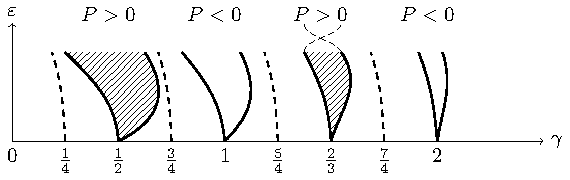
\includegraphics[scale=1.5]{img/parametric_oscillations/zones}
\end{figure}

Получились <<клювы>>, выходящие из последовательности точек на оси абсцисс. Таких точек бесконечное число. 

Зоны становятся уже с увеличением номера. Одно семейство образует $P^-$ зоны, лежащие в области $P<0$. Семейство в $P^+$ лежат в других областях. Во всех зонах реализуется параметрическая неустойчивость. В зонах, принадлежащих $P^-$, мультипликаторы нулевого состояния равновесия являются отрицательными, а в $P^+$ -- положительными.  

Вне этих зон будут либо периодические, либо квазипериодические колебания, в зависимости от параметра $\gamma$. Диссипация, если таковая имеется, приведет к тому, что глубины модуляции изменятся: зоны будут начинаться не с 0, а с некоторого $\varepsilon^*>0$. 
	
% \newpage
% \section{Динамика маятника с вибрирующей точкой подвеса. Маятник Капицы}
% \label{sec:kap_pendulum}
% 	% 29.04.19 
% 	%!TEX root = ../lections.tex

\begin{wrapfigure}[9]{l}{0.4\linewidth} 
\vspace{0.15em}
\centering
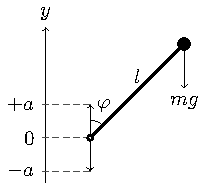
\includegraphics[scale=1.5]{img/kap_pendulum/kap_pendulum}
% \vspace{-0.25em}
% \caption{Some caption}
% \label{fig:somelabel}
\end{wrapfigure}
Рассмотрим шарик на упругом стержне, пренебрегая массой стержня. Точка подвеса колеблется с амплитудой $a$ и периодом $2\tau$. Изначально маятник расположен в верхнем положении равновесия. 


Пусть $\tau \ll 1$ (точка подвеса быстро осциллирует) и $l\gg a$.

Пусть точка подвеса совершает равнопеременные движения с ускорением $a \pm c$, тогда с каждым полупериодом $c=\frac{8a}{\tau^2}$, частота $\omega_p^2=\frac{c}{l}=\frac{8a}{l\tau^2}$. Считаем, что диссипации нет. 

Систему можно описать уравнениями:
\begin{equation}
	\left\{\begin{aligned}
		\dot{\varphi}=y \\
		\dot{y}=(\omega_0^2 \pm \omega_p^2)	\varphi,
	\end{aligned}\right.
	\label{eq:89}	
\end{equation}
где $\omega_0$ - собственная частота маятника, если бы не было колебаний подвеса. Знак $\pm$ изменяется через время $\tau$, $\omega_p^2>\omega_0^2$. Эта система параметрическая, к ней можно применить недавно рассмотренную теорию. 

Система  \eqref{eq:89} является кусочно-линейной. Построим матрицу $G$.

\paragraph{Матрица $G_1$.} Пусть в начальный момент точка подвеса в крайнем верхнем положении. Тогда в течение первого полупериода:
\begin{gather*}
	\dot{\varphi}=y,\quad
	\dot{y}=p^2\varphi,\quad
	p^2=\omega_0^2 + \omega_p^2.
\end{gather*}
$p$ действительные и разного знака. ФСР можно записать в виде:
\begin{gather}
	\phi_1(t)=\ch(pt),\quad \psi_1(t)=\frac1{p}\sh(pt), \notag \\ 
	\phi_2(t)=p\sh(pt),\quad \psi_2(t)=\ch(pt).		
	\label{eq:90}
\end{gather}
Тогда элементы матрицы будут
\begin{gather*}
	a_1=\ch(p\tau), c_1=\frac1{p}\sh(p\tau), \notag \\ 
	b_1=p\sh(p\tau), d_1=\ch(p\tau).		
\end{gather*}

\paragraph{Матрица $G_2$.} Будем считать, что маятник в нижнем положении и начинает движение вверх:
\begin{gather}
	\dot{\varphi}=y,\quad
	\dot{y}=p^2\varphi,\quad
	p^2=\omega_0^2 - \omega_p^2.
	\label{eq:91}
\end{gather}
Корни чисто мнимые. Фундаментальная система решений:
\begin{gather*}
	\phi_1(t)=\cos(\omega t),\quad \psi_1(t)=\frac1{\omega}\sin(\omega t), \notag \\ 
	\phi_2(t)=-\omega \sin(\omega t),\quad \psi_2(t)=\cos(\omega t).
\end{gather*}
Подставляя $\tau$, найдем:
\begin{gather*}
	a_1=\cos(\omega \tau), \quad c_1=\frac1{\omega}\sin(\omega \tau), \notag \\ 
	b_1=-\omega \sin(\omega \tau), \quad d_1=\cos(\omega \tau).		
\end{gather*}

Перемножаем $G_1 \cdot G_2$, получаем:
\begin{gather*}
	P=a+d=2\ch(p \tau)\cos(\omega \tau)+\qty(\frac{p}{\omega}-\frac{\omega}{p})\sh(p \tau)\sin(\omega \tau).		
\end{gather*}

Для устойчивости $|P|<1$. Получаем неравенство на параметры. Оно строилось численно, заданы: $a=0.1$см, $l=100$ см.

\begin{wrapfigure}[9]{l}{0.5\linewidth} 
	\vspace{0.1em}
	\centering
	\includegraphics[scale=1.5]{img/kap_pendulum/p_tau}
	\vspace{-0.25em}
\end{wrapfigure}

Существует интервал, где неравенство выполняется. В данном случае $\tau_s=0.006738$. Число колебаний $N=\frac{1}{2\tau}$. Если $N>678$ колебаний в секунду, то верхняя точка становится устойчивой. Внешнее воздействие превратило неустойчивое состояние равновесия в высокочастотное колебание вблизи состояния равновесия.





\subsection{Колебания линейного осциллятора с медленно меняющейся частотой}
Рассмотрим линейный осциллятор:
\begin{gather}
	\ddot{x}+\omega_0^2(\mu t)x=0, \qq{где} \omega_0(\mu t)>0,~0< \mu \ll t
	\label{eq:92}
\end{gather}
Введём новое время $\tau=\mu t$, тогда
\begin{gather}
	\left\{\begin{aligned}
		&\mu \dv{x}{\tau}=y \\
		&\mu \dv{y}{\tau}=-\omega_0^2(\tau)x.
	\end{aligned}\right.	
	\label{eq:93}
\end{gather}
Для исследования используем метод Вентцеля-Крамерса-Бриллюэна (ВКБ). В соответствии с ним, будем искать решение в виде:
\begin{gather}
	\left\{\begin{aligned}
		x=e^{\frac{s(\tau)}{\mu}}\sum\limits_{j=0}^{\infty}\mu^j u_j(\tau) \\
		y=e^{\frac{s(\tau)}{\mu}}\sum\limits_{j=0}^{\infty}\mu^j v_j(\tau),
	\end{aligned}\right.	
	\label{eq:94}
\end{gather}
где $s(\tau),~u_j(\tau),~v_j(\tau)$ - неизвестные функции, которые надо найти. 

Будем искать решение нулевого порядка по $\mu$:
\begin{gather}
	\left\{\begin{aligned}
		x=e^{\frac{s(\tau)}{\mu}}\qty[u_0(\tau)+\mu u_1(\tau)] \\
		y=e^{\frac{s(\tau)}{\mu}}\qty[v_0(\tau)+\mu v_1(\tau)].
	\end{aligned}\right.	
	\label{eq:95}
\end{gather}
Подставляем \eqref{eq:95} в \eqref{eq:93} и группируем слагаемые по порядку $\mu$:
\begin{equation}
	\mu^0:
	\left\{\begin{aligned}
		&\dv{s}{\tau} u_0(\tau)-v_0(\tau)=0 \\
		&\omega^2_0(\tau)u_0(\tau)+\dv{s}{\tau} v_0(\tau)=0, 		
	\end{aligned}\right.
	\label{eq:96}	
\end{equation}
\begin{equation}
	\mu^1:
	\left\{\begin{aligned}
		&\dv{s}{\tau} u_1(\tau)+\dv{u_0}{\tau}=v_1(\tau) \\
		&\dv{s}{\tau} v_1(\tau)+\dv{v_0}{\tau}=-\omega^2_0(\tau)u_1(\tau). 		
	\end{aligned}\right.
	\label{eq:97}	
\end{equation}

Система \eqref{eq:96} представляет собой СЛАУ относительно $u_0$, $v_0$. Из условия равенства нулю определителя системы получим
\begin{equation}
	\qty(\dv{s}{\tau})^2+\omega^2_0(\tau)=0,
	\label{eq:98}	
\end{equation}
\begin{equation}
	\dv{s}{\tau}=\pm i\omega_0(\tau),
	\label{eq:99}	
\end{equation}

Проинтегрируем:
\begin{gather}
	s(\tau)=\pm i \int_0^{\tau}\omega_0(\tau)\dd \tau, \qq{тогда} ~u_0=\psi(\tau), ~v_0=\pm i \omega_0(\tau)\psi(\tau), 
	\label{eq:100}
\end{gather}
где $\psi(\tau)$ -- ввели произвольную функцию (просто переобозначили $u_0(\tau)$).

Уравнение \eqref{eq:100} определяет пару комплексно сопряженных решений. Рассмотрим с <<$+$>>:
\begin{equation}
	v_1(\tau)=\dv{s}{\tau}u_1(\tau)+\dv{\psi}{\tau}.
	\label{eq:101}	
\end{equation}
Подставляя \eqref{eq:100} и \eqref{eq:101} в \eqref{eq:97}, получим:
\begin{equation}
	2\omega_0(\tau)\dv{\psi}{\tau}=-\psi\dv{\omega_0(\tau)}{\tau}.
	\label{eq:102}	
\end{equation}
В \eqref{eq:102} переменные разделяются. Проинтегрируем:
\begin{equation*}
	\psi(\tau)=\frac{A}{\sqrt{\omega_0(\tau)}}.
\end{equation*}
Чтобы составить полное решение, нужно проделать ту же процедуру для знака <<$-$>>. В итоге получим
\begin{equation*}
	x(\tau) \approx \frac{A}{\sqrt{\omega_0(\tau)}} \exp \qty[\frac{i}{\mu}\int_0^{\tau}\omega_0(\tau)\dd \tau]+\frac{A}{\sqrt{\omega_0(\tau)}} \exp \qty[-\frac{i}{\mu}\int_0^{\tau}\omega_0(\tau)\dd \tau],
\end{equation*}
или, возвращаясь к исходному времени
\begin{gather}
	x(t) \approx \frac{2A}{\sqrt{\omega_0(\mu t)}}\cos\vartheta, \qq{где}
	\vartheta=\int_0^{\mu \tau}\omega_0(t)\dd t
	\label{eq:103s}
\end{gather}

Найдем полную энергию осциллятора:
\begin{equation}
	E=\frac{(\dot x)^2}{2}+\omega_0^2(\mu t)\frac{x^2}{2}, 
	\label{eq:104}
\end{equation}
\begin{equation}
	\dot{x}=-\frac{A\cos\vartheta \cdot \dot{\omega}(\mu t)}{\omega_0(\mu t)\sqrt{\omega_0(\mu t)}}-\frac{2A\sin\vartheta \cdot \omega_0(\mu t)}{\sqrt{\omega_0(\mu t)}}.
	\label{eq:105}	
\end{equation}
В первом приближении $\dot \omega \approx 0$, поэтому формула упрощается:
\begin{equation}
	\dot{x}=-2A\sqrt{\omega_0(\mu t)}\sin\vartheta.
	\label{eq:106}	
\end{equation}
Подставим \eqref{eq:103s}, \eqref{eq:106} в \eqref{eq:104}:
\begin{equation*}
	E \approx A^2 \omega_0(\mu t).
\end{equation*}
Энергия меняется пропорционально частоте изменения осциллятора:
\begin{equation*}
	\frac{E}{\omega_0(\mu t)}=const.
\end{equation*}

Увеличивая частоту, увеличиваем и энергию. А отношение их есть \textbf{адиабатический} (т.к. медленно меняем частоту) \textbf{инвариант}. 

Итак, мы рассмотрели линейные параметрические системы: резонансные (условия параметрического резонанса), быстро осциллирующие и медленно осциллирующие.


% \newpage
% \section{Введение в теорию многомерных динамических систем}
% \label{sec:multidimensional_dynamic_systems}
% % 29.04.19 
% 	Под многомерными динамическими системами понимаются системы, размерность фазового пространства которых равна трем и выше. 
\begin{wrapfigure}[9]{l}{0.75\linewidth} 
	\vspace{0.1em}
	\centering
	\includegraphics[scale=1]{fig/fig48.pdf}
	\vspace{-0.25em}
\end{wrapfigure}
Для систем на плоскости задача была разбить плоскость параметров на области с разными характеристическими бифуркационными линиями.

На фазовой плоскости существовало конечное число предельных циклов и состояний равновесия.

Многомерные системы делятся на 2 класса:
\begin{enumerate}
	\item Системы с конечным числом состояний равновесия, периодических движений и числом бифуркаций. Такие системы носят название систем Морса-Смейла. Они есть подобие двумерных систем.
	\item Системы с бесконечным числом периодических движений и бифуркаций. 
\end{enumerate}

Интересны бифуркации, при которых один класс переходит в другой.

\subsection{Основные бифуркации состояний равновесия трехмерных систем}
Запишем систему:
\begin{equation}
	\begin{cases}
		\dot x = P(x, y, z, \mu) \\
		\dot y = Q(x, y, z, \mu) \\
		\dot z = R(x, y, z, \mu),
	\end{cases}
	\label{eq:107}	
\end{equation}

Без ограничения общности, будем считать, что состояние равновесия в начале координат $O_0(x=y=z=\mu=0),~\mu \in [-\mu_0,\mu_0]$.

\textit{Двукратное равновесие:}

$\lambda_1(0)=0,~Re[\lambda_{2,3}(\mu)] \neq 0$

Перепишем, приведя систему к нормальному виду:
\begin{gather*}
	\dot U_1 = \mu+lU_1^2+\dots, \\
	\dot V=\beta(\mu)V+\dots, \\
	V=
	\begin{pmatrix}
		U_2 \\
		U_3
	\end{pmatrix}
	.
\end{gather*}

\underline{Случай а:}
\begin{gather*}
	\beta(\mu)=
	\begin{pmatrix}
		\lambda_2~~0 \\
		0~~\lambda_3
	\end{pmatrix}
	.
\end{gather*}

Случай аналогичен седлоузлу в двумерной системе. Условие невырожденности: $l\neq 0$,
\begin{gather*}
	\beta(\mu)=
	\begin{cases}
		\dot U_1 = \mu+lU_1^2+\dots \\
		\dot U_2 = \lambda_2U_2+\dots \\
		\dot U_3 = \lambda_3U_3+\dots.
	\end{cases}
\end{gather*}

Пусть $\lambda_2,~\lambda_3<0,~l>0,~U_1^2=-\frac{\mu}{l}$:
\begin{figure}[H]
	\centering
	\includegraphics[width=1\linewidth]{fig/fig49.pdf}   
\end{figure}

При $\mu<0$ - устойчивый узел и седло с одномерной сепаратрисой. При $\mu=0$ седлоузел - негрубое состояние равновесия, которое при изменении параметра либо распадается на два, либо исчезает. 

\underline{Случай b:}
\begin{gather*}
	\lambda_{2,3}=\alpha(\mu)\pm i \beta(\mu), \\
	\beta(\mu)=
	\begin{pmatrix}
		\alpha~~-\beta \\
		\beta~~~~\alpha
	\end{pmatrix}
	.
\end{gather*}

Предполагаем, что $Re[\alpha(\mu)]<0$.
\begin{gather*}
	\beta(\mu)=
	\begin{cases}
		\dot U_1 = \mu+lU_1^2+\dots \\
		\dot U_2 = \alpha U_2-\beta U_3 \\
		\dot U_3 = \beta U_2+\alpha U_3.
	\end{cases}
\end{gather*}
\begin{figure}[H]
	\centering
	\includegraphics[width=1\linewidth]{fig/fig50.pdf}   
\end{figure}

При $\mu<0$ - устойчивый фокус и седлофокус. При $\mu=0$ седлофокус-фокус.

Пусть корни все действительные. $\lambda_3<0,~\lambda_2>0,~\mu<0$. Для удобства расположим оси координат следующим образом:
\begin{wrapfigure}[6]{l}{0.5\linewidth} 
	\vspace{0.1em}
	\centering
	\includegraphics[scale=1]{fig/fig51.pdf}
	\vspace{-0.25em}
\end{wrapfigure}

Одно седло имеет одномерную сепаратрису и двумерное устойчивое многообразие, другое - одно неустойчивое двумерное многообразие и устойчивое одномерное.

\begin{figure}[H]
	\centering
	\includegraphics[width=1\linewidth]{fig/fig52.pdf}   
\end{figure}

Многообразия пересекаются, сближаются. Образуется точка, которая при $\mu>0$ исчезает.

27.05
\subsection{Бифуркация коразмерности 1 Андронова-Хопфа}
Предположим, есть состояние равновесия. Его корни комплексно-сопряженные: $\lambda_{1,2}=\alpha(\mu)\pm i \beta(\mu),~\beta(\mu)>0,~\mu=0$ - бифуркационный параметр, который состоит в том, что $\alpha(0)=0$. Условие невырожденности - первая ляпуновская величина $L(\mu)\neq 0$.

Рассмотрим конкретный вид зависимости:
\begin{wrapfigure}[7]{l}{0.42\linewidth} 
	\vspace{0.1em}
	\centering
	\includegraphics[scale=1]{fig/fig53.pdf}
	\vspace{-0.25em}
\end{wrapfigure}

$\lambda_3(\mu)\neq 0,~L(\mu)<0$,
\begin{equation}
	\begin{cases}
		\dot U_1 = \alpha(\mu)U_1-\beta(\mu)U_2+L(\mu)(U_1^2+U_2^2)U_1+\dots \\
		\dot U_2 = \beta(\mu)U_1+\alpha(\mu)U_2+L(\mu)(U_1^2+U_2^2)U_2+\dots \\
		\dot U_3 = \lambda_3(\mu)U_3+\dots
	\end{cases}
	\label{eq:108}	
\end{equation}

 Для определенности $\lambda_3(\mu)<0$ (рассмотреть $\lambda_3(\mu)>0$).

 Фактически, для рассмотрения такой системы нам достаточно знаний о двумерных системах. Из третьего уравнения системы находим, что $U_3=0$ - инвариантная плоскость. Без третьего уравнения остается двумерная система. Легко восстановить фазовые портреты:
 \begin{figure}[H]
	\centering
	\includegraphics[width=1\linewidth]{fig/fig54.pdf}   
\end{figure}

При $\mu=0$ состояние равновесия не центр, а сложный устойчивый фокус. В этом случае динамику системы определяют кубические слагаемые. При $\mu>0$ появляется предельный устойчивый цикл. 

$\lambda_3<0,~U_3 \rightarrow 0$. $U_3$ - устойчивая плоскость (если рассмотреть одномерную систему на прямой).

\begin{center}
    \begin{minipage}{0.32\linewidth}
        \includegraphics[width=\linewidth]{fig/55_1.jpg} 
        \vspace{-50pt}
        \label{fig:1}
    \end{minipage}
\hfill     
    \begin{minipage}{0.3\linewidth}
        \includegraphics[width=\linewidth]{fig/55_2.jpg} 
        \vspace{-50pt}
        \label{fig:1}
    \end{minipage}
\hfill     
    \begin{minipage}{0.3\linewidth}
        \includegraphics[width=\linewidth]{fig/55_3.jpg} 
        \vspace{-50pt}
        \label{fig:1}
    \end{minipage}    
\end{center}

Справа - неустойчивый седлофокус.

$L>0:$
\begin{figure}[H]
	\centering
	\includegraphics[width=1\linewidth]{fig/fig58.pdf}   
\end{figure}

\begin{center}
    \begin{minipage}{0.32\linewidth}
        \includegraphics[width=\linewidth]{fig/fig61.jpg} 
        \vspace{-50pt}
        \label{fig:1}
    \end{minipage}
\hfill     
    \begin{minipage}{0.3\linewidth}
        \includegraphics[width=\linewidth]{fig/fig60.jpg} 
        \vspace{-50pt}
        \label{fig:1}
    \end{minipage}
\hfill     
    \begin{minipage}{0.3\linewidth}
        \includegraphics[width=\linewidth]{fig/fig59.jpg} 
        \vspace{-50pt}
        \label{fig:1}
    \end{minipage}    
\end{center}

Слева седловой предельный цикл, по центру - точка стала неустойчивым сложным фокусом.

\subsection{Бифуркации периодических движений в трехмерном пространстве(бифуркация +1)}
Предположим, есть система третьего порядка, в которой существует предельный цикл $L_{\mu}$, зависящий от $\mu$. Для введения мультипликатора выберем произвольную точку, через нее проведем секущую Пуанкаре. Мультипликаторов три, один из которых тривиальный: $s_1(\mu),~s_2(\mu)$.
\begin{wrapfigure}[7]{l}{0.6\linewidth} 
	\vspace{0.1em}
	\centering
	\includegraphics[scale=1]{fig/fig62.pdf}
	\vspace{-0.25em}
\end{wrapfigure}

Первое - седло-узловая бифуркация предельных циклов (двукратный предельный цикл). Предположим, $s_j(\mu)>0$, и при $\mu<0$ оба мультипликатора расположены внутри единичной окружности. При этом $0<s_2(\mu)<1$.
\begin{figure}[H]
	\centering
	\includegraphics[width=1\linewidth]{fig/fig63.pdf}   
\end{figure}

При $\mu=0: s_1(0)= 1$. Запишем нормальную форму для этой бифуркации. На секущей Пуанкаре вводятся координаты. Тогда поведение вблизи $L_{\mu}$ может быть описано двумерным отображением:
\begin{equation}
	\begin{cases}
		\stackrel{\_}{\xi}= \mu+\xi+\xi^2+\dots \equiv g\\
		\stackrel{\_}{\eta}= s_2(\mu)\eta+\dots
	\end{cases}
	\label{eq:109}	
\end{equation}

Переменные $\xi, \eta$ вводятся в малой $\varepsilon$-окрестности предельного цикла. $\mu$ близко к 0.

g может быть исследовано независимо. Неподвижные точки $\stackrel{\_}{\xi}=\xi$:
$$\xi^2+\mu=0.$$

При $\mu<0: \xi^2=-\mu~\rightarrow \xi=\pm \sqrt{-\mu}$.

Устойчивость:
\begin{gather*}
	g'_{\xi}=1+2\xi, \\
	g''_{\xi \xi}=2,
\end{gather*}
$\xi$ мало, следовательно, $g'_{\xi}>0$. Функция монотонно растет и выпукла вниз.
\begin{figure}[H]
	\centering
	\includegraphics[width=1\linewidth]{fig/fig64.pdf}   
\end{figure}

При $\mu=0 g'=1, s_1=1$ - точка полуустойчивая. 

Из второго уравнения системы получаем, что $\eta=0$ - инвариантная прямая. Любая точка, взятая на этой прямой, перепрыгнет на нее же. Она устойчива:  
\begin{figure}[H]
	\centering
	\includegraphics[width=1\linewidth]{fig/fig65.pdf}   
\end{figure}

Слева направо: на вертикальных прямых действует второе отображение. На них траектории стремятся к $\eta=0$. Затем остается одна неподвижная точка - седлоузел (это не равновесие, а отображение). После чего исчезает.

Это все отображения, т.е набор точек (нарисовано сплошными).
\begin{figure}[H]
	\centering
	\includegraphics[width=1\linewidth]{fig/fig66.pdf}   
\end{figure}

Слева устойчивый (внешний) и седловой (внутренний) предельные циклы. Им соответствуют неподвижные точки. По центру негрубая неподвижная точка и двукратный предельный цикл. Справа - нет предельного цикла.

\subsection{Бифуркация удвоения периода (бифуркация -1)}
Пусть мультипликаторы отрицательные:
\begin{figure}[H]
	\centering
	\includegraphics[width=1\linewidth]{fig/fig67.pdf}   
\end{figure}

Динамику поведения в окрестности предельного цикла можно описать нормальной формой:
\begin{equation}
	\begin{cases}
		\stackrel{\_}{\xi}= -(1+\mu)\xi+\xi^3+\dots \equiv g(\xi,\mu)\\
		\stackrel{\_}{\eta}= s_2(\mu)\eta+\dots
	\end{cases}
	\label{eq:110}	
\end{equation}

Первое уравнение можно исследовать отдельно. Мультипликаторы отрицательны, следовательно, будут перескоки. 

Удобнее начать с отображения $\stackrel{=}{\xi}$, т.е. посмотреть, как ведет себя система через две итерации.
\begin{gather*}
	\stackrel{=}{\xi}=-(1+\mu)\stackrel{\_}{\xi}+\stackrel{\_}{\xi}^3+\dots= \\
	=-(1+\mu)(-(1+\mu)\xi+\xi^3)+(-(1+\mu)\xi+\xi^3)^3+\dots= \\
	=(1+\mu)^2\xi-(1+\mu)\xi^3-(1+\mu)^3\xi^3+\dots=(1+\mu)^2\xi-(1+\mu)((1+\mu)^2+1)\xi^3+\dots
\end{gather*}

Найдем неподвижные точки:



\end{document}
